%!TEX root = ../thesis.tex
%*******************************************************************************
%****************************** Third Chapter **********************************
%*******************************************************************************
\chapter{Data and analysis}

% **************************** Define Graphics Path **************************
\ifpdf
    \graphicspath{{Chapter3/Figs/Raster/}{Chapter3/Figs/PDF/}{Chapter3/Figs/}}
\else
    \graphicspath{{Chapter3/Figs/Vector/}{Chapter3/Figs/}}
\fi

\section[SEM Data]{SEM Data}
\label{section3.1}

\subsection[Azurite and blue verditer]{Azurite and blue verditer}
\label{subsection3.1.1}

This section discusses qualitatively the morphological features, regularity, and approximate particle size of the reference samples described in \textit{Table \ref{table:ref_sample}}.  
% ************************************************     HKI nat az sample     *******************************************************************

\textit{Figures \ref{fig:hki_nat_az_sem_1}-\ref{fig:hki_nat_az_sem_5}} show the sample HKI natural azurite. This sample is of unknown date and provenance but is confirmed to be naturally produced, which offers a baseline against which to compare other samples known to be synthetic or of unknown origin. Maginification ranges from 250x to 4000x. Significant surface charging was not observed with this sample.

In \textit{Figure \ref{fig:hki_nat_az_sem_1}}, two areas are shown at 250x magnification. Particle sizes are very irregular, as are shapes and volumes. Particles appear to be relatively flat-sided rather than rough. 

\begin{figure}[H]
\centering
\begin{minipage}{.45\textwidth}
  \centering
  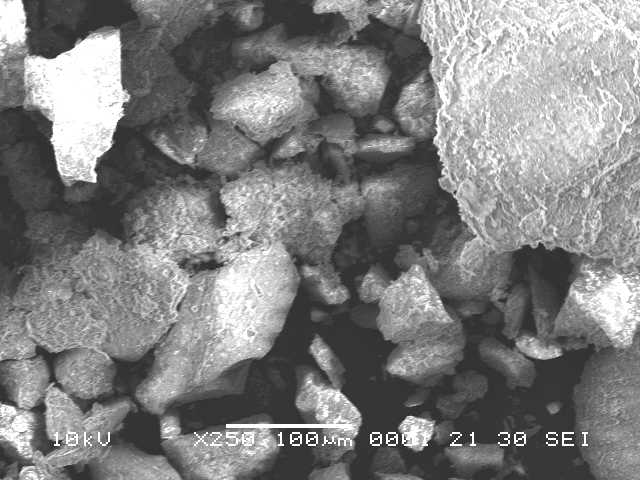
\includegraphics[width=\linewidth]{HKI_natural_azurite_x250_3_040521}
\end{minipage}
\begin{minipage}{.45\textwidth}
  \centering
  \includegraphics[width=\linewidth]{HKI_natural_azurite_x250_5_040521}
\end{minipage}
\caption[SEM images: Sample HKI, natural azurite]{SEM images: Sample HKI, natural azurite. Magnification: 250x.}
\label{fig:hki_nat_az_sem_1}
\end{figure}

It is possible to see the surface texture of larger particles more clearly at 750x magnification in \textit{Figure \ref{fig:hki_nat_az_sem_2}}. It appears that there are smaller particles embedded in or settled on the surface of larger particles, making a rough surface. Particles have clearly sharp angular edges and are not rounded. At this magnification the large variation in particle size is apparent, and the asymmetry of the material is noted.

\begin{figure}[H]
\centering
\begin{minipage}{.45\textwidth}
  \centering
  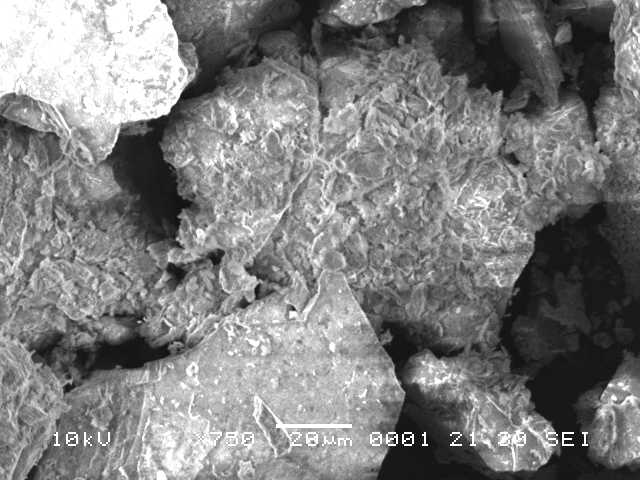
\includegraphics[width=\linewidth]{HKI_natural_azurite_x750_1_040521}
\end{minipage}
\begin{minipage}{.45\textwidth}
  \centering
  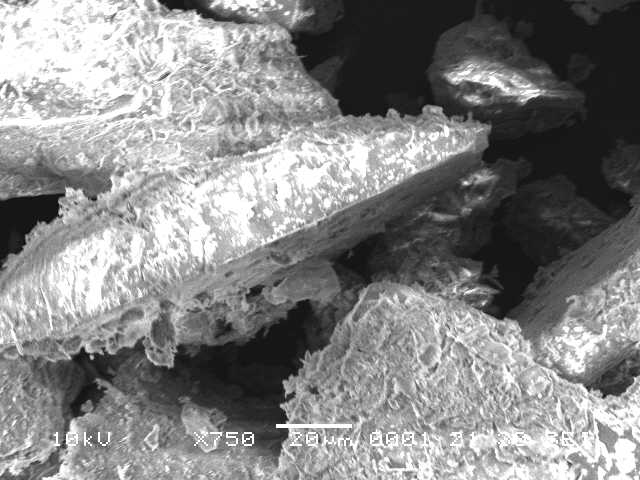
\includegraphics[width=\linewidth]{HKI_natural_azurite_x750_3_040521}
\end{minipage}
\caption[SEM images: Sample HKI, natural azurite]{SEM images: Sample HKI, natural azurite. Magnification: 750x.}
\label{fig:hki_nat_az_sem_2}
\end{figure}

The fine surface detail on the flat sides of larger particles can be observed at 1500x magnification in \textit{Figure \ref{fig:hki_nat_az_sem_3}}. The image on the right shows several more spherical looking particles, though many more appear asymmetrical with uneven sharp edges. The size of the texture on the surface is consistent in size in contrast to the macro size heterogeneity.

\begin{figure}[H]
\centering
\begin{minipage}{.45\textwidth}
  \centering
  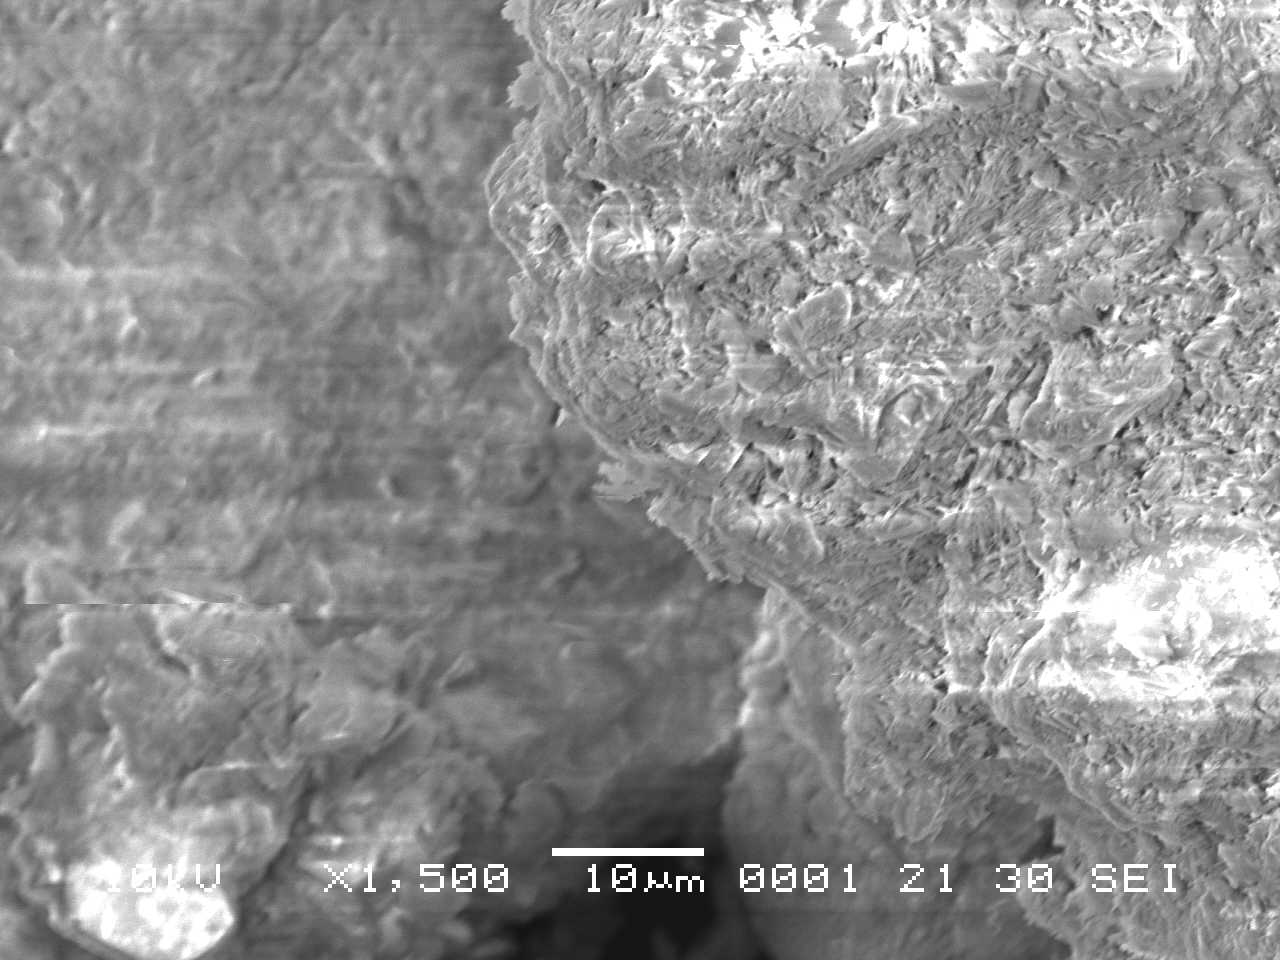
\includegraphics[width=\linewidth]{HKI_natural_azurite_x1500_2_040521}
\end{minipage}
\begin{minipage}{.45\textwidth}
  \centering
  \includegraphics[width=\linewidth]{HKI_natural_azurite_x1500_4_040521}
\end{minipage}
\caption[SEM images: Sample HKI, natural azurite]{SEM images: Sample HKI, natural azurite. Magnification: 1500x.}
\label{fig:hki_nat_az_sem_3}
\end{figure}

\textit{Figure \ref{fig:hki_nat_az_sem_4}} shows two images at 2000x magnification. The image on the right shows clear sharp-sided particles. These are extremely uneven. The left image, on the other hand, shows flat irregular small particles layered over one another like flakes.

\begin{figure}[H]
\centering
\begin{minipage}{.45\textwidth}
  \centering
  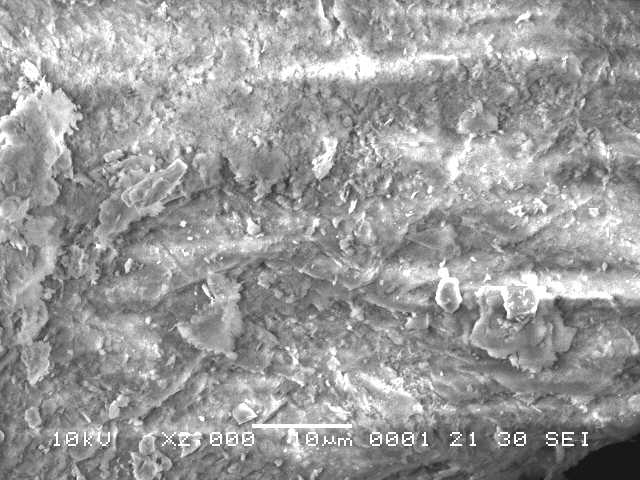
\includegraphics[width=\linewidth]{HKI_natural_azurite_x2000_1_040521}
\end{minipage}
\begin{minipage}{.45\textwidth}
  \centering
  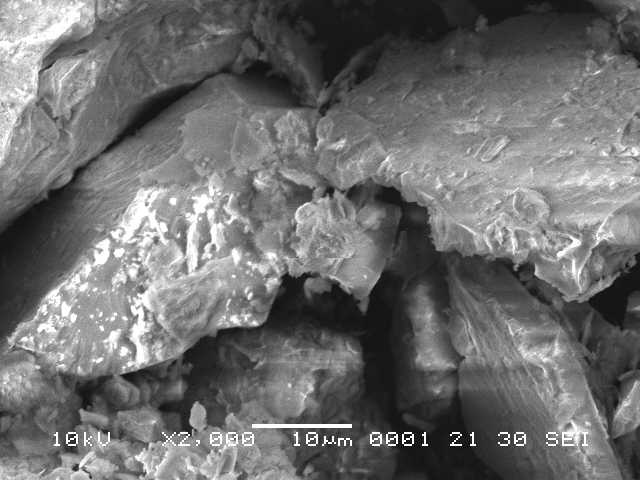
\includegraphics[width=\linewidth]{HKI_natural_azurite_x2000_3_040521}
\end{minipage}
\caption[SEM images: Sample HKI, natural azurite]{SEM images: Sample HKI, natural azurite. Magnification: 2000x.}
\label{fig:hki_nat_az_sem_4}
\end{figure}

At very high magnification (4000x), \textit{Figure \ref{fig:hki_nat_az_sem_5}} shows the fine structure of the sample very clearly. There is still significant size variation at this magnification, and interesting needle like crystal formations are observed. These do appear to be orientated in some places, possibly showing the areas of crystal nucleation and growth. Other needle like crystals appear randomly orientated. Notably, this ordering is not readily observed in other samples, though needle like crystals are.

\begin{figure}[H]
\centering
\begin{minipage}{.45\textwidth}
  \centering
  \includegraphics[width=\linewidth]{HKI_natural_azurite_x4000_2_040521}
\end{minipage}
\begin{minipage}{.45\textwidth}
  \centering
  \includegraphics[width=\linewidth]{HKI_natural_azurite_x4000_5_040521}
\end{minipage}
\caption[SEM images: Sample HKI, natural azurite]{SEM images: Sample HKI, natural azurite. Magnification: 4000x.}
\label{fig:hki_nat_az_sem_5}
\end{figure}

% ************************************************     Az1     *******************************************************************

Sample Az1, likely from a natural source, is shown in \textit{Figures \ref{fig:az1_sem_1}} and \textit{\ref{fig:az1_sem_2}}. 

\textit{Figure \ref{fig:az1_sem_1}}, at 750x magnification, shows significant size variation in the sample. There are many flat, sharp particles as well as many smaller particles. It is difficult to determine whether the larger pieces of sample are aggregates of smaller particles or larger intact pieces; the surfaces of these appear almost pocked, especially in the left image.

\begin{figure}[H]
\centering
\begin{minipage}{.45\textwidth}
  \centering
  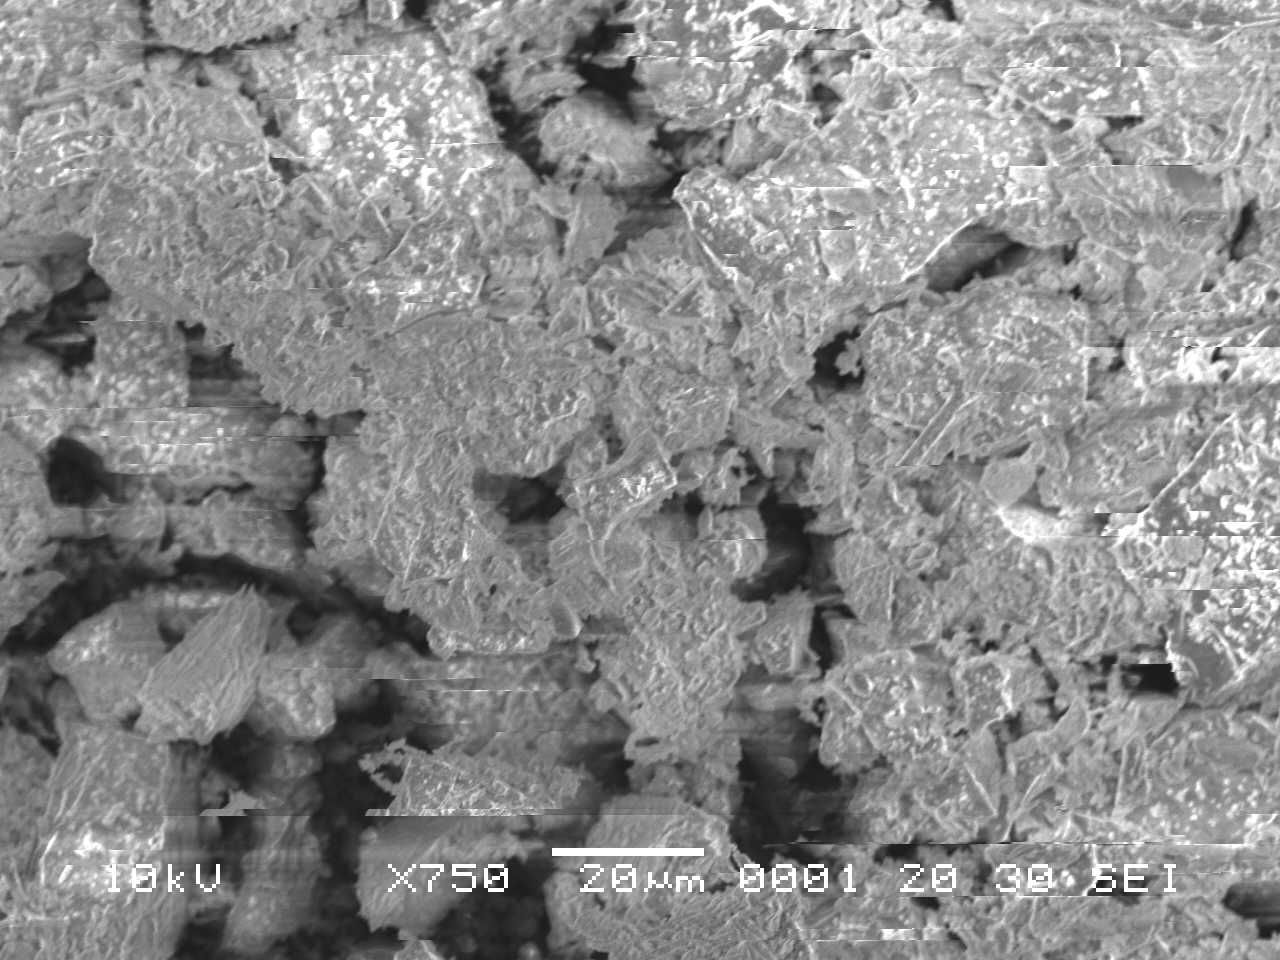
\includegraphics[width=\linewidth]{Az1_x750_3_220221}
\end{minipage}
\begin{minipage}{.45\textwidth}
  \centering
  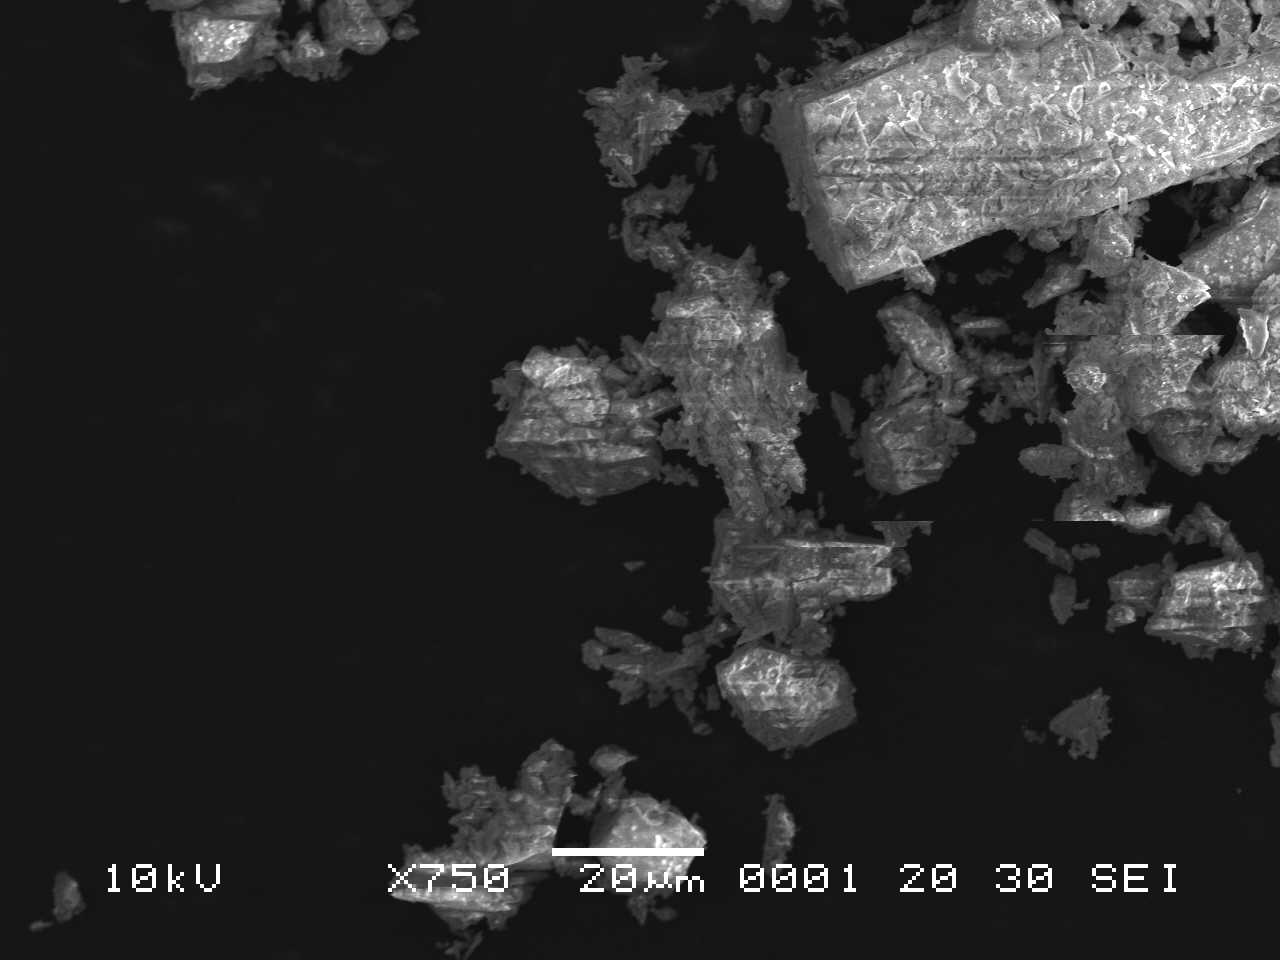
\includegraphics[width=\linewidth]{Az1_x750_6_220221}
\end{minipage}
\caption[SEM images: Sample Az1, azurite]{SEM images: Sample Az1, azurite. Magnification: 750x.}
\label{fig:az1_sem_1}
\end{figure}

\textit{Figure \ref{fig:az1_sem_2}} shows Az1 at 1500x (left) and 2000x (right). At 1500x, it is possible to observe smaller voluminous (not flat) particles on the surface of larger particles. The vast majority of pieces are irregularly shaped with choppy borders, though a few circular particles are also present. At 2000x, the image shows the flat edge of a larger particle. There is a great deal of surface texture, as well as some intriguing grid formations that do not appear to be artifacts of the SEM. These may be due to grinding and polishing of the pigment, but also may suggest some crytal ordering. Uniformity of shape and size is low at all magnifications and all over the sample.

\begin{figure}[H]
\centering
\begin{minipage}{.45\textwidth}
  \centering
  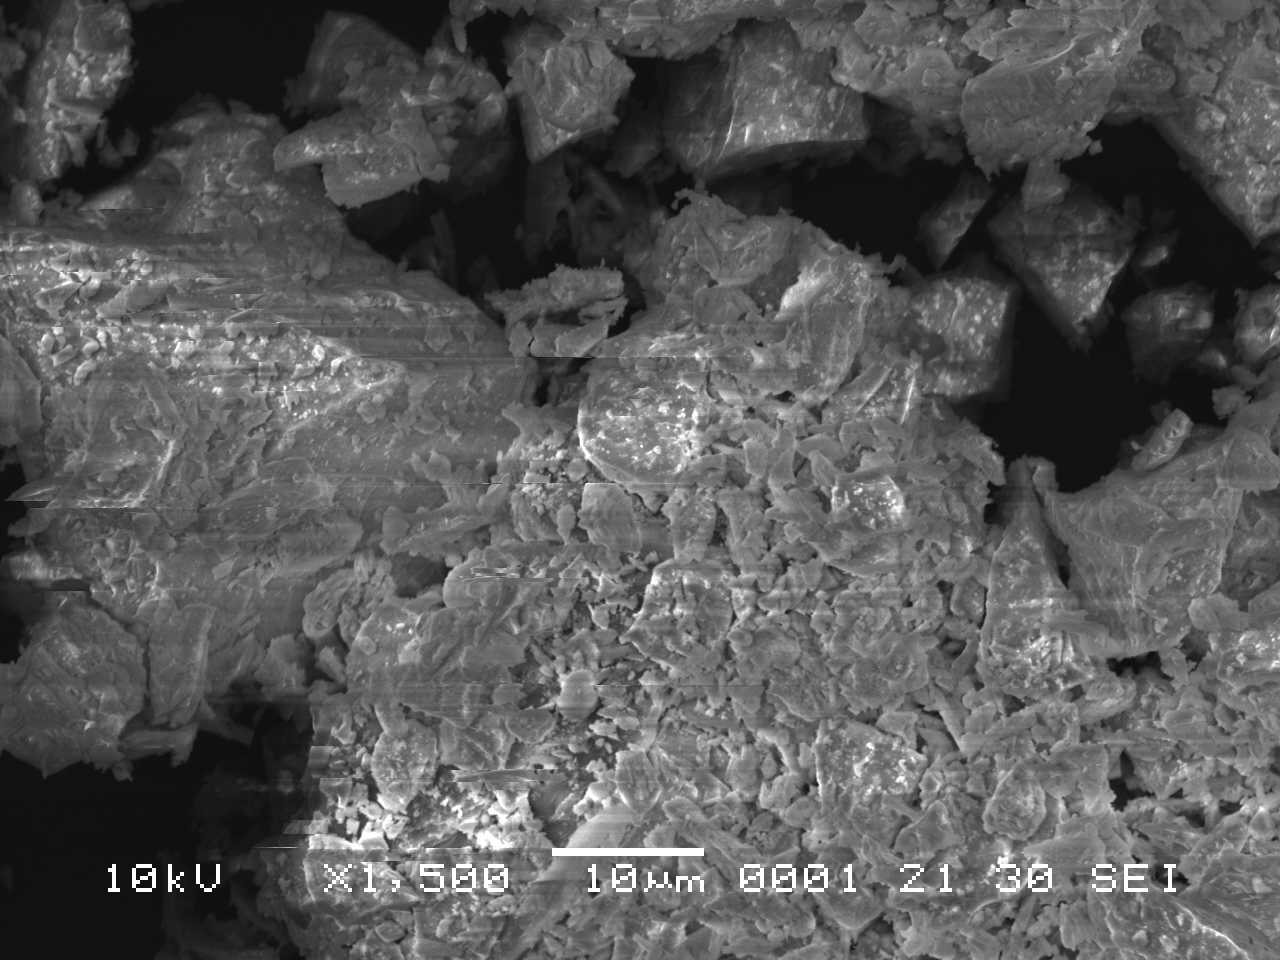
\includegraphics[width=\linewidth]{Az1_x1500_2_220221}
\end{minipage}
\begin{minipage}{.45\textwidth}
  \centering
  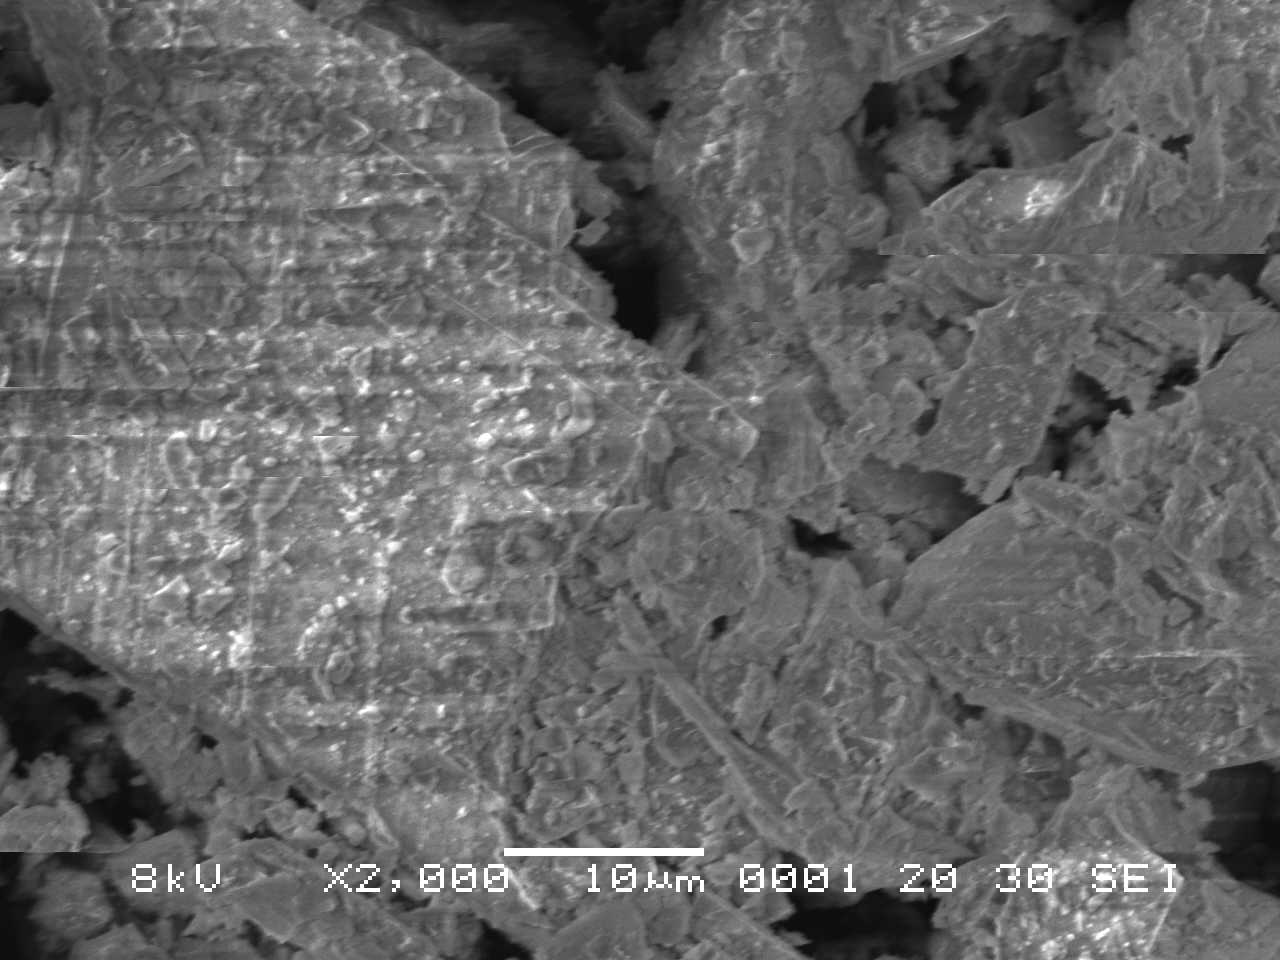
\includegraphics[width=\linewidth]{Az1_x2000_4_220221}
\end{minipage}
\caption[SEM images: Sample Az1, azurite]{SEM images: Sample Az1, azurite. Magnification: \textbf{left)} 1500x, \textbf{right)} 2000x}
\label{fig:az1_sem_2}
\end{figure}

% ************************************************     Az2     *******************************************************************

\textit{Figures \ref{fig:az2_sem_1}} and \textit{\ref{fig:az2_sem_2}} show sample Az2, which is morphologically significantly different from all other observed samples and lacks the features that appear to correlate with either natural or artificial pigment sources. Surface charging made it difficult to image this sample, and this issue was also not observed with most other samples.

In \textit{Figure \ref{fig:az2_sem_1}}, two images of the sample at 200x magnification are shown. It is interesting that although the shape of each sample is quite asymmetric and angular, the size and irregular shape is quite consistent between particules. At this magnification, the surface of the particles appears flat and smooth. It is also significant that these particles are much larger than the average particle size observed in other samples, which may suggest industrial pigment grinding. Otherwise, this consistency could also reflect a synthetic origin, with controlled conditions of crystal growth.

\begin{figure}[H]
\centering
\begin{minipage}{.45\textwidth}
  \centering
  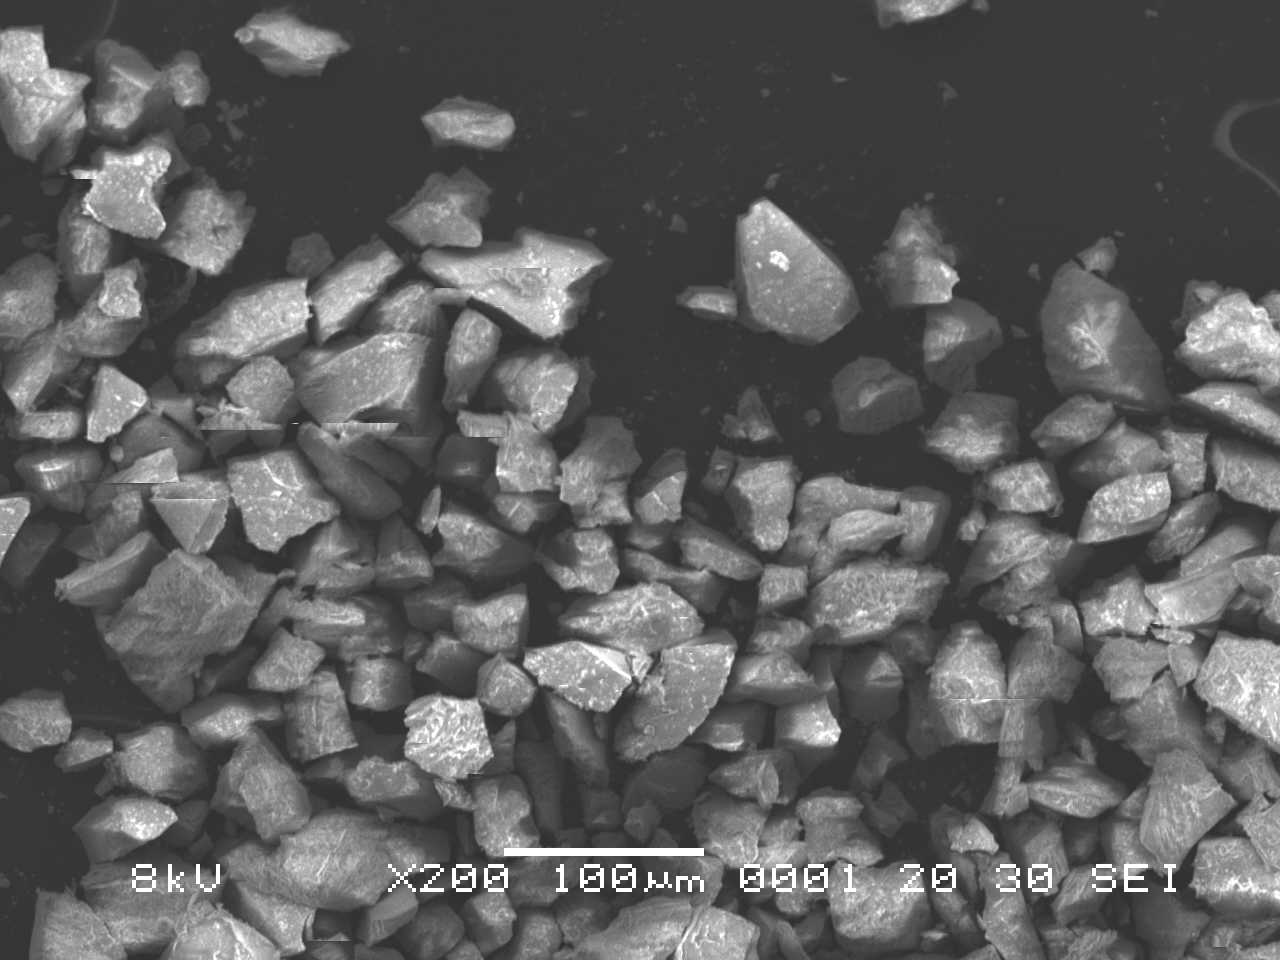
\includegraphics[width=\linewidth]{Az2_x200_1_240221}
\end{minipage}
\begin{minipage}{.45\textwidth}
  \centering
  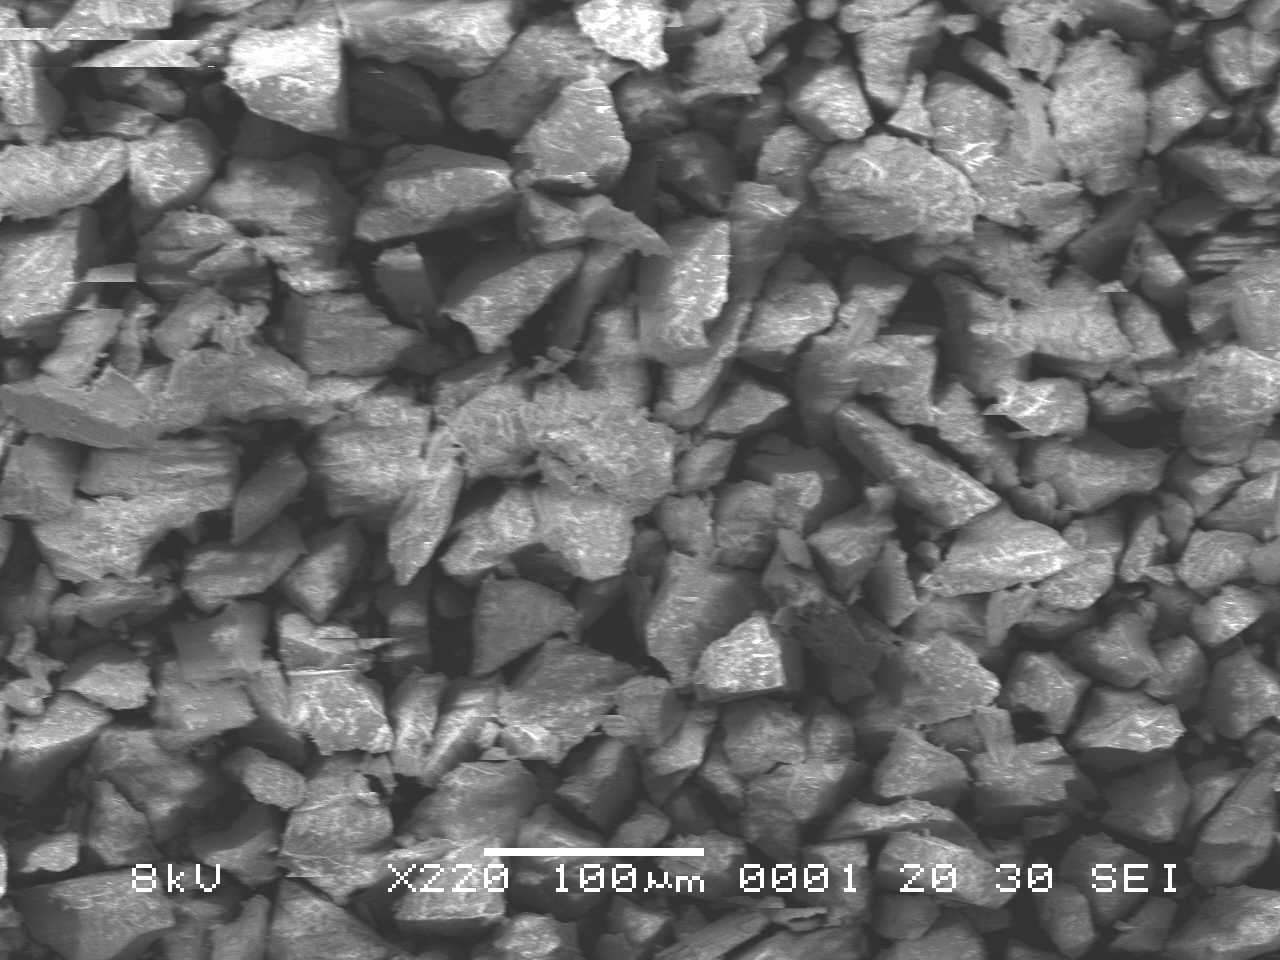
\includegraphics[width=\linewidth]{Az2_x200_2_240221}
\end{minipage}
\caption[SEM images: Sample Az2, azurite]{SEM images: Sample Az2, azurite. Magnification: 200x.}
\label{fig:az2_sem_1}
\end{figure}

In \textit{Figure \ref{fig:az2_sem_2}}, Az2 is shown at 750x (left) and 1500x (right). Imaging at higher magnifications was not possible due to charging. At 750x magnification, relatively flat sides of particles are observed. There is slightly more size variation than initially seen, though this is difficult to assess due to jumping of particles during charging. At 1500x magnification, there is very little surface texture observed. Sample Az2 is obviously unlike the sample HKI natural azurite. However, it also does not resemble known synthetic samples either. 

\begin{figure}[H]
\centering
\begin{minipage}{.45\textwidth}
  \centering
  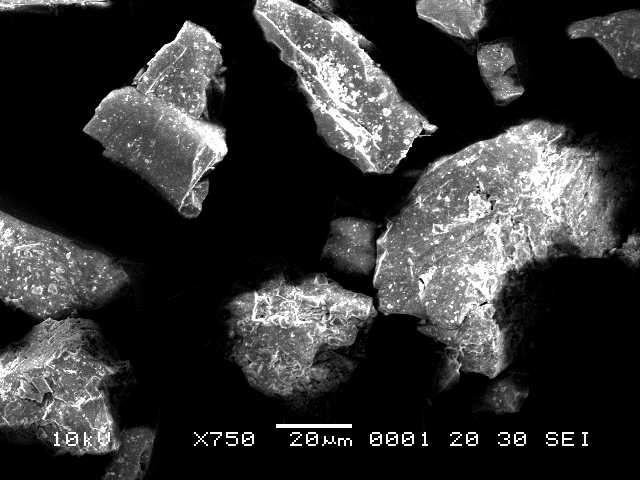
\includegraphics[width=\linewidth]{Az2_x750_1_150321}
\end{minipage}
\begin{minipage}{.45\textwidth}
  \centering
  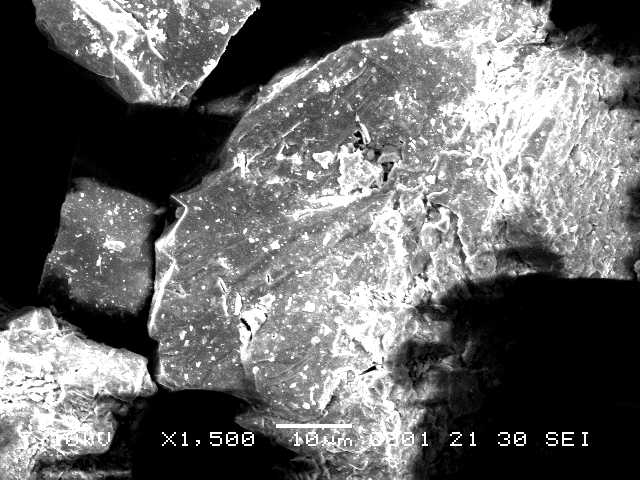
\includegraphics[width=\linewidth]{Az2_x1500_1_150321}
\end{minipage}
\caption[SEM images: Sample Az2, azurite]{SEM images: Sample Az2, azurite. Magnification: \textbf{left)} 750x, \textbf{right)} 1500x}
\label{fig:az2_sem_2}
\end{figure}

% ************************************************     AzMag     *******************************************************************

\textit{Figures \ref{fig:azmag_sem_1}-\ref{fig:azmag_sem_5}} show sample AzMag at magnifications from 200x to 4000x. 

At 200-250x magnification (\textit{Figure \ref{fig:azmag_sem_1}}), extremely small particles are shown. The particle size is fairly homogeneous, though there is a great deal of variation in particle shape as well as a lot of texture observed.

\begin{figure}[H]
\centering
\begin{minipage}{.45\textwidth}
  \centering
  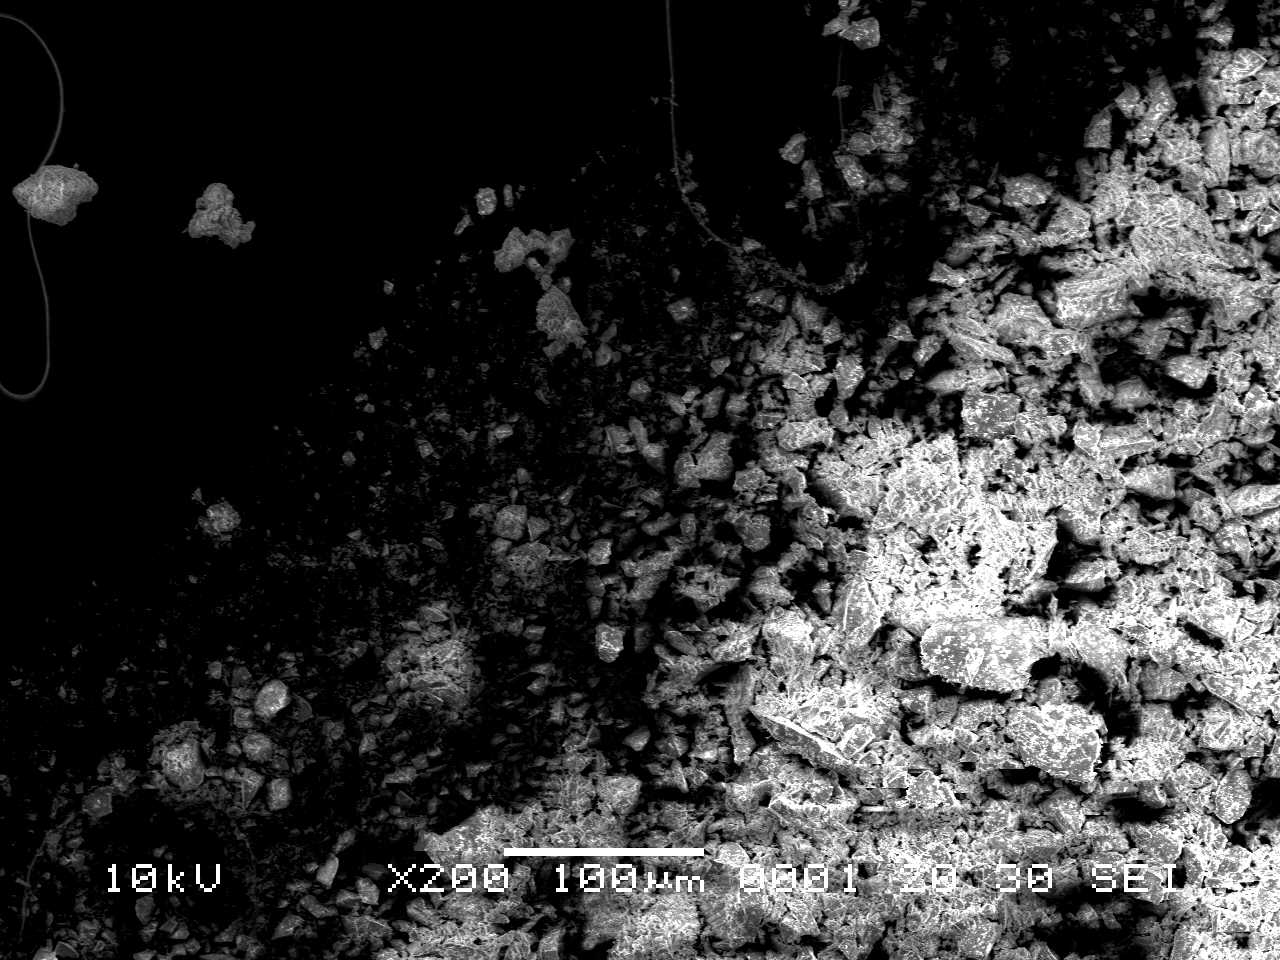
\includegraphics[width=\linewidth]{AzMag_x200_1_260221}
\end{minipage}
\begin{minipage}{.45\textwidth}
  \centering
  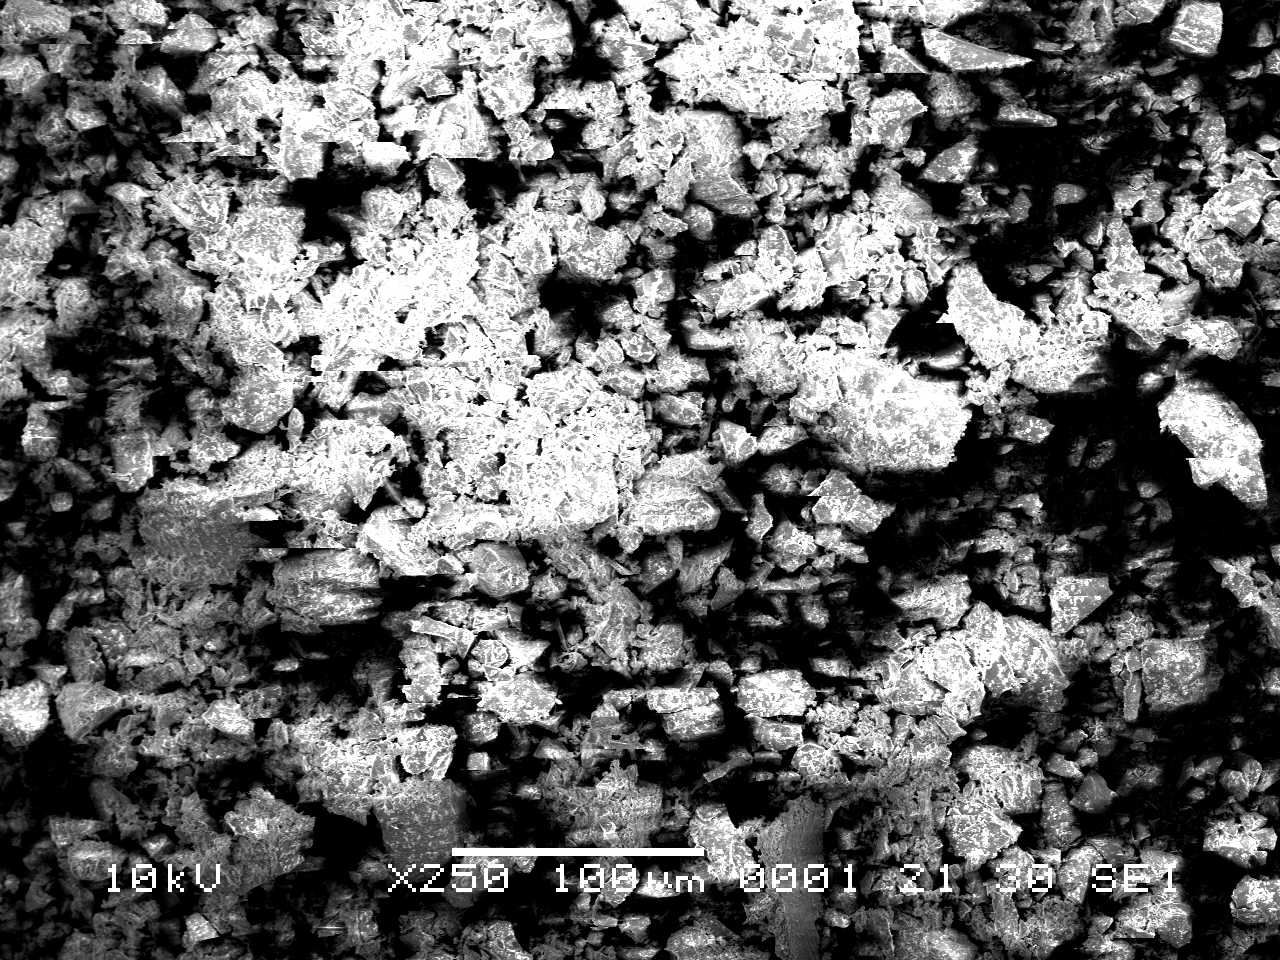
\includegraphics[width=\linewidth]{AzMag_x250_2_160321}
\end{minipage}
\caption[SEM images: Sample AzMag, azurite]{SEM images: Sample AzMag, azurite. Magnification: \textbf{left)} 200x, \textbf{right)} 250x}
\label{fig:azmag_sem_1}
\end{figure}

\textit{Figure \ref{fig:azmag_sem_2}} shows the sample at 750x magnification. The surfaces are choppy, rough, and highly textured. Most particles are approximately square or triangular, with a few small spheres on the surface. Elongated and large particles are not observed.

\begin{figure}[H]
\centering
\begin{minipage}{.45\textwidth}
  \centering
  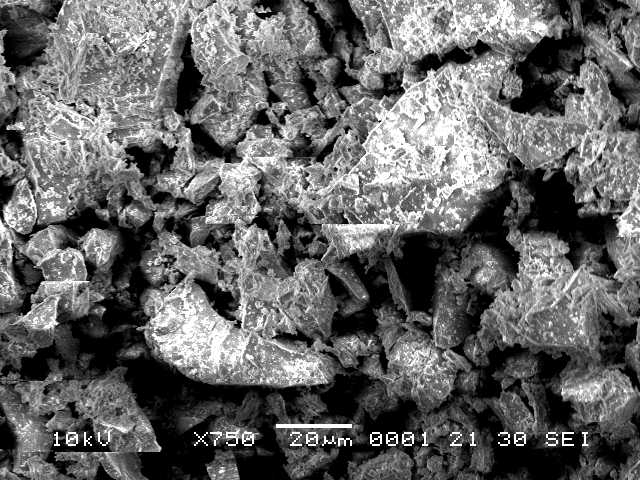
\includegraphics[width=\linewidth]{AzMag_x750_1_160321}
\end{minipage}
\begin{minipage}{.45\textwidth}
  \centering
  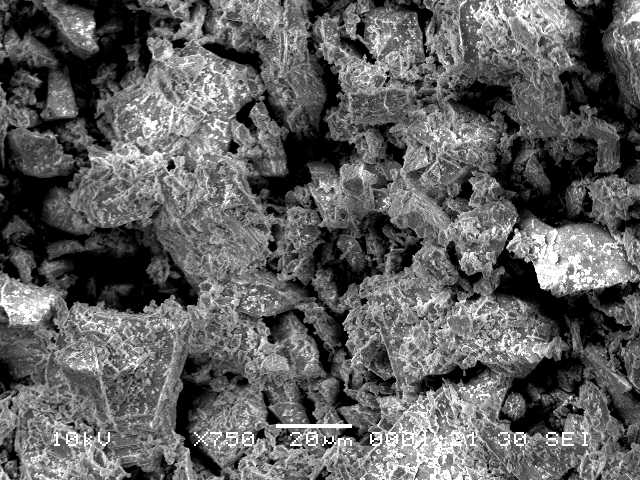
\includegraphics[width=\linewidth]{AzMag_x750_3_160321}
\end{minipage}
\caption[SEM images: Sample AzMag, azurite]{SEM images: Sample AzMag, azurite. Magnification: 750x}
\label{fig:azmag_sem_2}
\end{figure}

\textit{Figure \ref{fig:azmag_sem_3}} and the left image in \textit{Figure \ref{fig:azmag_sem_4}} show the sample at 1500x magnification. Here, sample AzMag is qualitatively similar to HKI natural azurite. There are thinnner forms, though they are not quite as delicate as the needle like formations discussed previously. 

\begin{figure}[H]
\centering
\begin{minipage}{.45\textwidth}
  \centering
  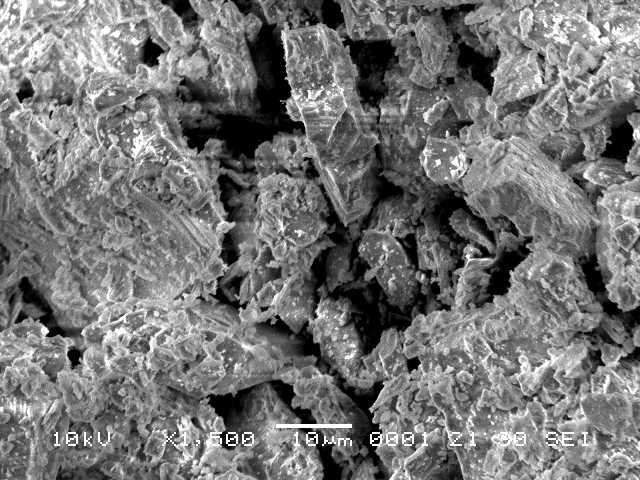
\includegraphics[width=\linewidth]{AzMag_x1500_1_160321}
\end{minipage}
\begin{minipage}{.45\textwidth}
  \centering
  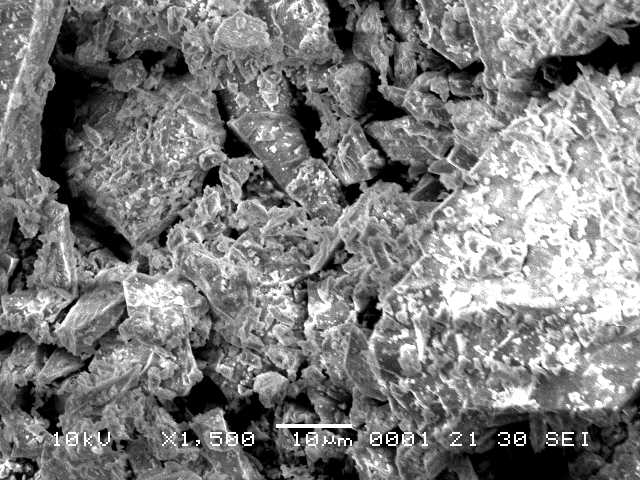
\includegraphics[width=\linewidth]{AzMag_x1500_3_160321}
\end{minipage}
\caption[SEM images: Sample AzMag, azurite]{SEM images: Sample AzMag, azurite. Magnification: 1500x}
\label{fig:azmag_sem_3}
\end{figure}

\begin{figure}[H]
\centering
\begin{minipage}{.45\textwidth}
  \centering
  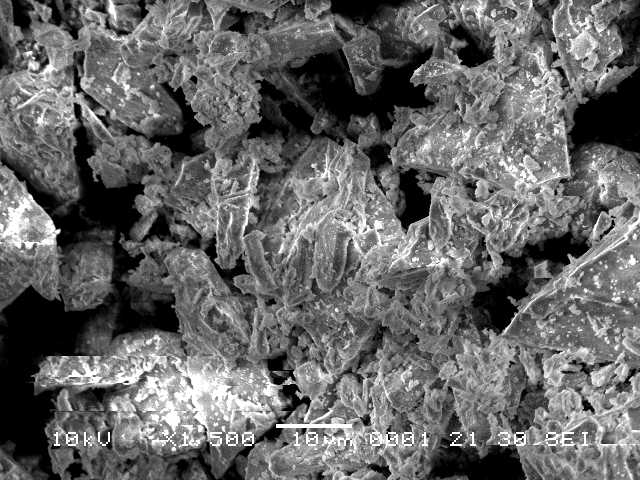
\includegraphics[width=\linewidth]{AzMag_x1500_5_160321}
\end{minipage}
\begin{minipage}{.45\textwidth}
  \centering
  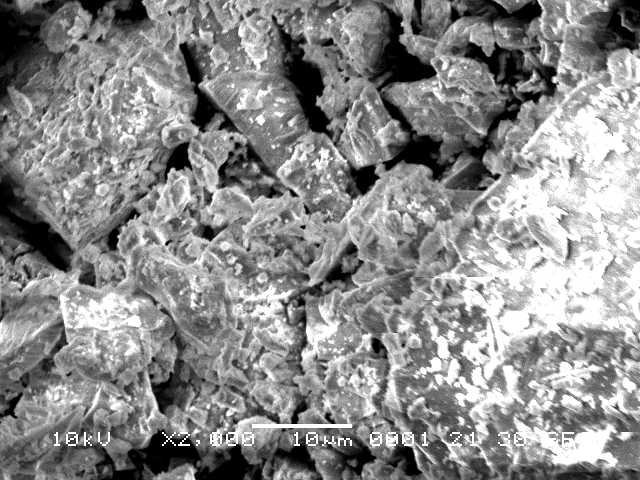
\includegraphics[width=\linewidth]{AzMag_x2000_1_160321}
\end{minipage}
\caption[SEM images: Sample AzMag, azurite]{SEM images: Sample AzMag, azurite. Magnification: \textbf{left)} 1500x, \textbf{right)} 2000x}
\label{fig:azmag_sem_4}
\end{figure}

At high magnification, the surface texture of the sample is clearly visualized. \textit{Figure \ref{fig:azmag_sem_5}} shows elongated, narrow crystals at 3000x (left) and 4000x (right). The directionality observed in HKI natural azurite at high magnifications is not observed here. However, the degree of roughness and character of the surfaces is very similar, implying that this sample is naturally produced.

\begin{figure}[H]
\centering
\begin{minipage}{.45\textwidth}
  \centering
  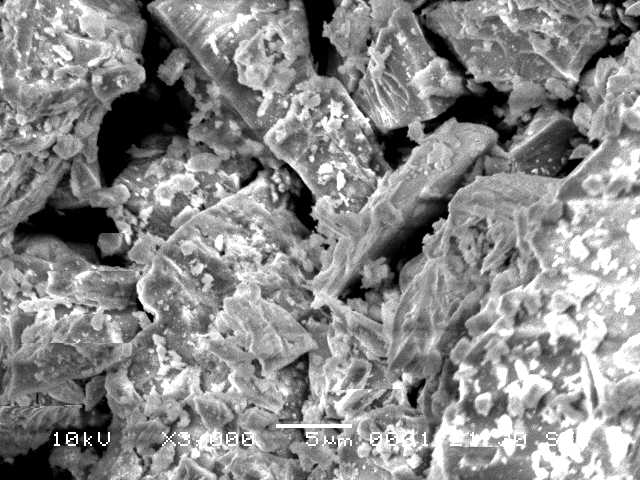
\includegraphics[width=\linewidth]{AzMag_x3000_1_160321}
\end{minipage}
\begin{minipage}{.45\textwidth}
  \centering
  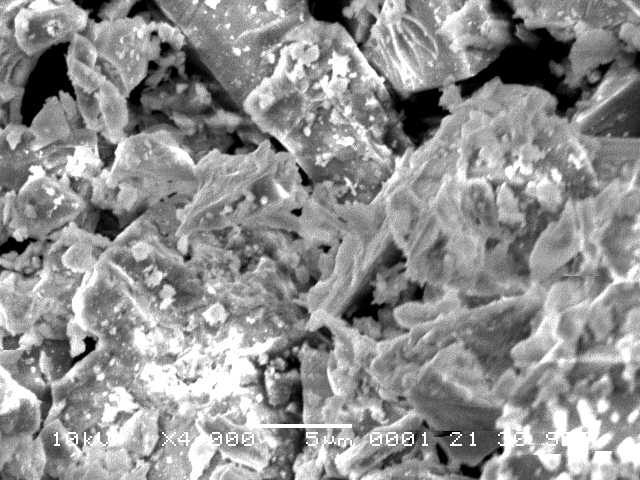
\includegraphics[width=\linewidth]{AzMag_x4000_1_160321}
\end{minipage}
\caption[SEM images: Sample AzMag, azurite]{SEM images: Sample AzMag, azurite. Magnification: \textbf{left)} 3000x, \textbf{right)} 4000x}
\label{fig:azmag_sem_5}
\end{figure}

% ************************************************     AzOp     *******************************************************************

\textit{Figures \ref{fig:azop_sem_1}-\ref{fig:azop_sem_3}} show sample AzOp at magnifications from 250x to 2000x. 

At 250x magnification (\textit{Figure \ref{fig:azop_sem_1}}, left), small and very textured particles are observed. The size of these particles is fairly homogenous. At 750x magnification (\textit{Figure \ref{fig:azop_sem_1}}, right), it is clear that there are larger particles/aggregations. It is difficult to tell whether these are in fact single pieces or clumps of smaller particles. The shape of all particles is extremely asymmetrical and varied, except in one specific case; at the bottom of the image there is a cluster of fairly uniformly spherical particles. 

\begin{figure}[H]
\centering
\begin{minipage}{.45\textwidth}
  \centering
  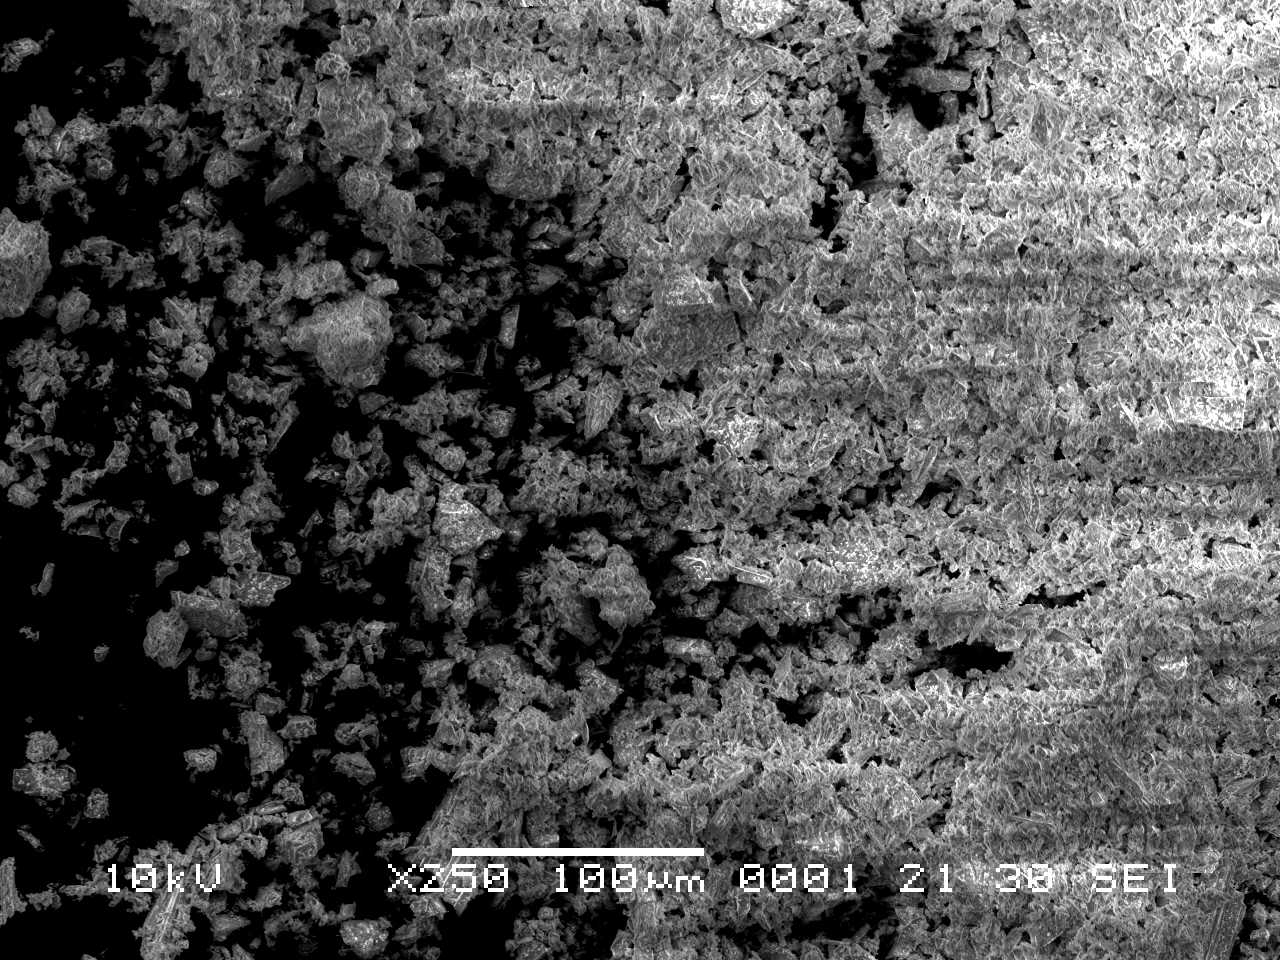
\includegraphics[width=\linewidth]{AzOp_x250_1_150321}
\end{minipage}
\begin{minipage}{.45\textwidth}
  \centering
  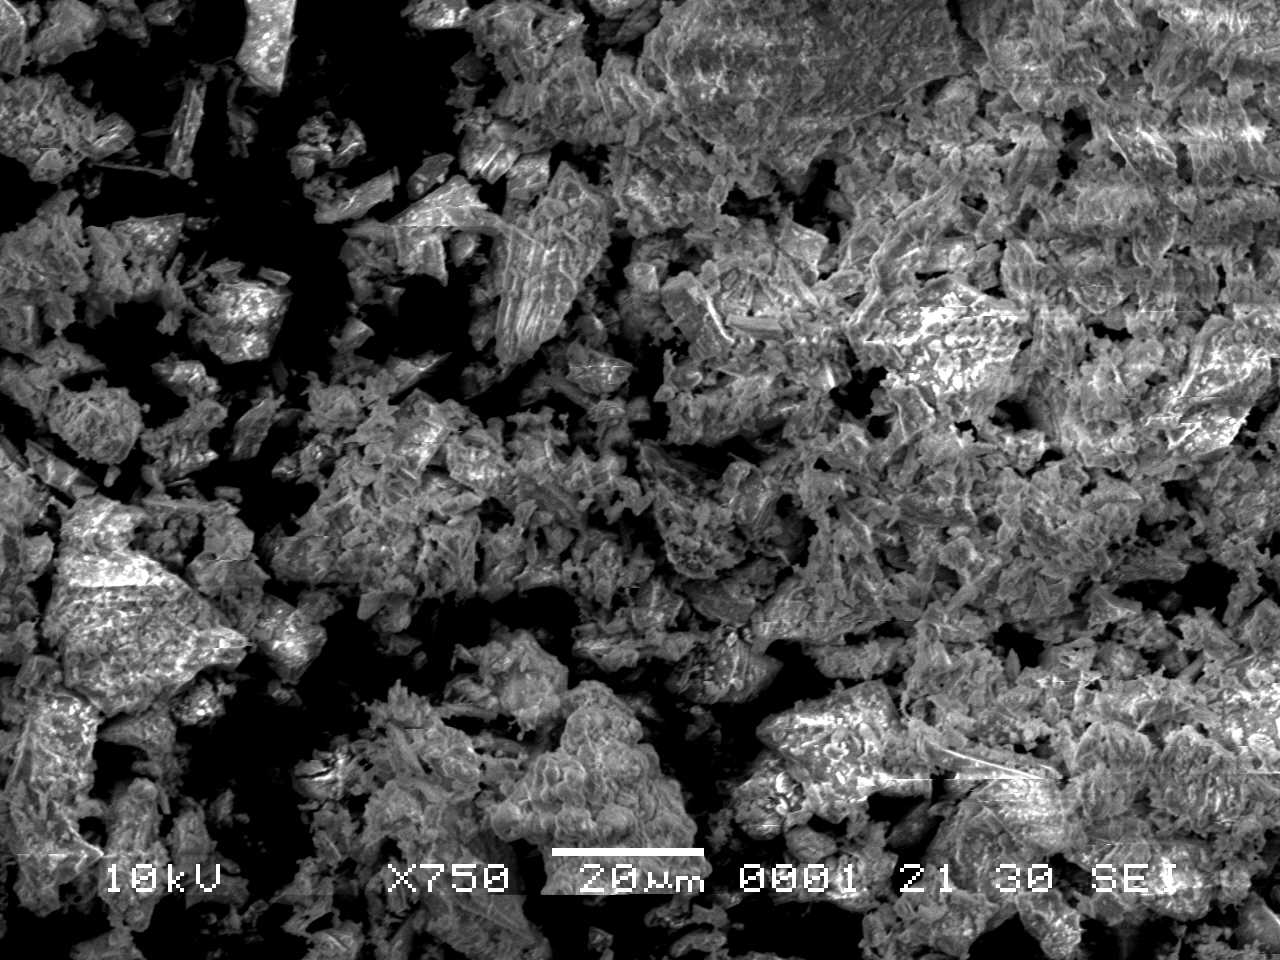
\includegraphics[width=\linewidth]{AzOp_x750_2_150321}
\end{minipage}
\caption[SEM images: Sample AzOp, azurite]{SEM images: Sample AzOp, azurite. Magnification: \textbf{left)} 250x, \textbf{right)} 750x}
\label{fig:azop_sem_1}
\end{figure}

The spherical particles are clearly observed in \textit{Figure \ref{fig:azop_sem_2}}, left, and \textit{Figure \ref{fig:azop_sem_3}}, right. They appear bubbly, as if many partial spheres have formed one on top of the other. This texture is not observed extensively in this sample, nor in other samples such as AzMag and HKI natural azurite that are otherwise similar to the rest of sample AzOp. This could be the result of sample contamination, as several samples were analyzed at the same time, or this could be evidence of multiple conditions under which crystals formed before being mixed to make this pigment. Regardless, this type of morphology is quite uniform and does not look like the result of random crushing and grinding. This certainly must be investigated further by imaging over a larger area of this sample as well as by preparing additional fresh samples.

In contrast, the rougher and more heterogenous texture of the majority of the sample is shown at 2000x magnification in \textit{Figure \ref{fig:azop_sem_3}}, left, and at 4000x magnification in \textit{Figure \ref{fig:azop_sem_2}}, right. Very few remotely circular particles are seen, and there is a great deal of heterogeneity in size and shape. This is very similar to natural samples discussed above.

\begin{figure}[H]
\centering
\begin{minipage}{.45\textwidth}
  \centering
  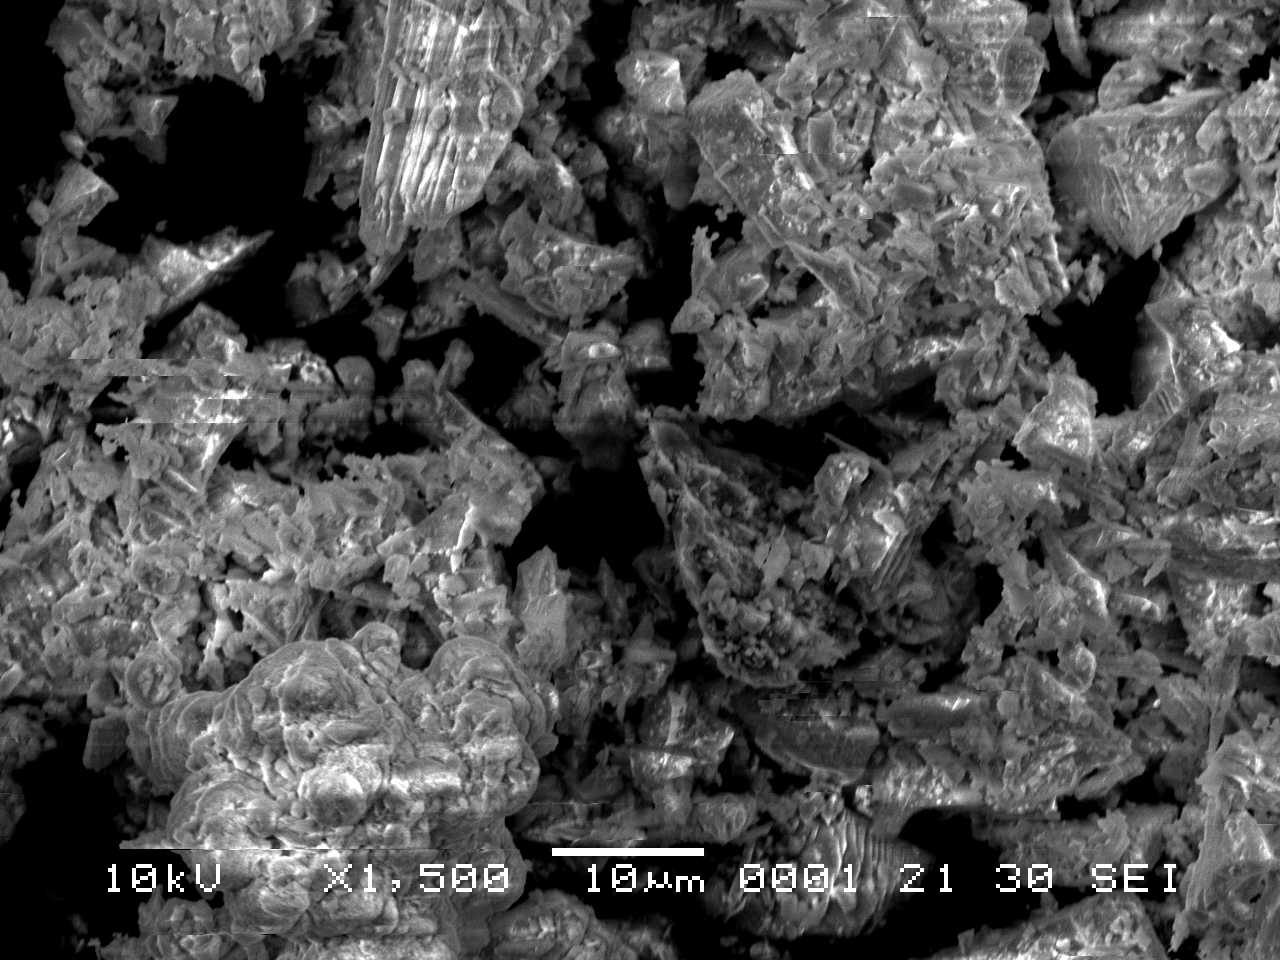
\includegraphics[width=\linewidth]{AzOp_x1500_2_150321}
\end{minipage}
\begin{minipage}{.45\textwidth}
  \centering
  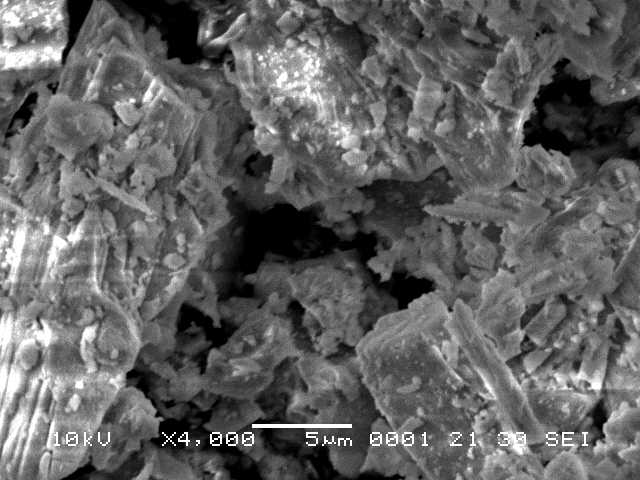
\includegraphics[width=\linewidth]{AzOp_x4000_1_150321}
\end{minipage}
\caption[SEM images: Sample AzOp, azurite]{SEM images: Sample AzOp, azurite. Magnification: \textbf{left)} 1500x, \textbf{right)} 4000x}
\label{fig:azop_sem_2}
\end{figure}

\begin{figure}[H]
\centering
\begin{minipage}{.45\textwidth}
  \centering
  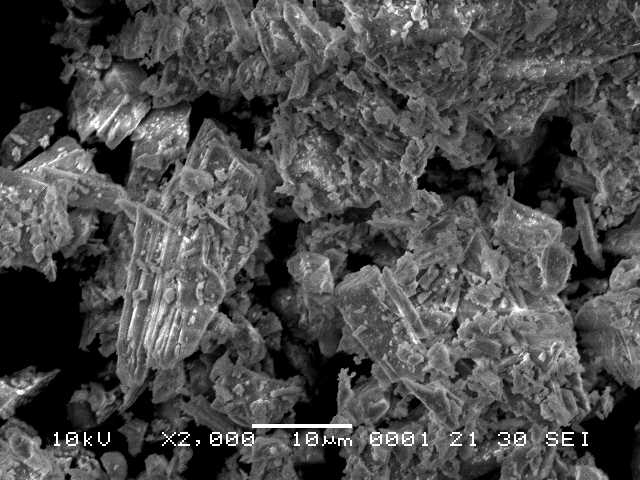
\includegraphics[width=\linewidth]{AzOp_x2000_1_150321}
\end{minipage}
\begin{minipage}{.45\textwidth}
  \centering
  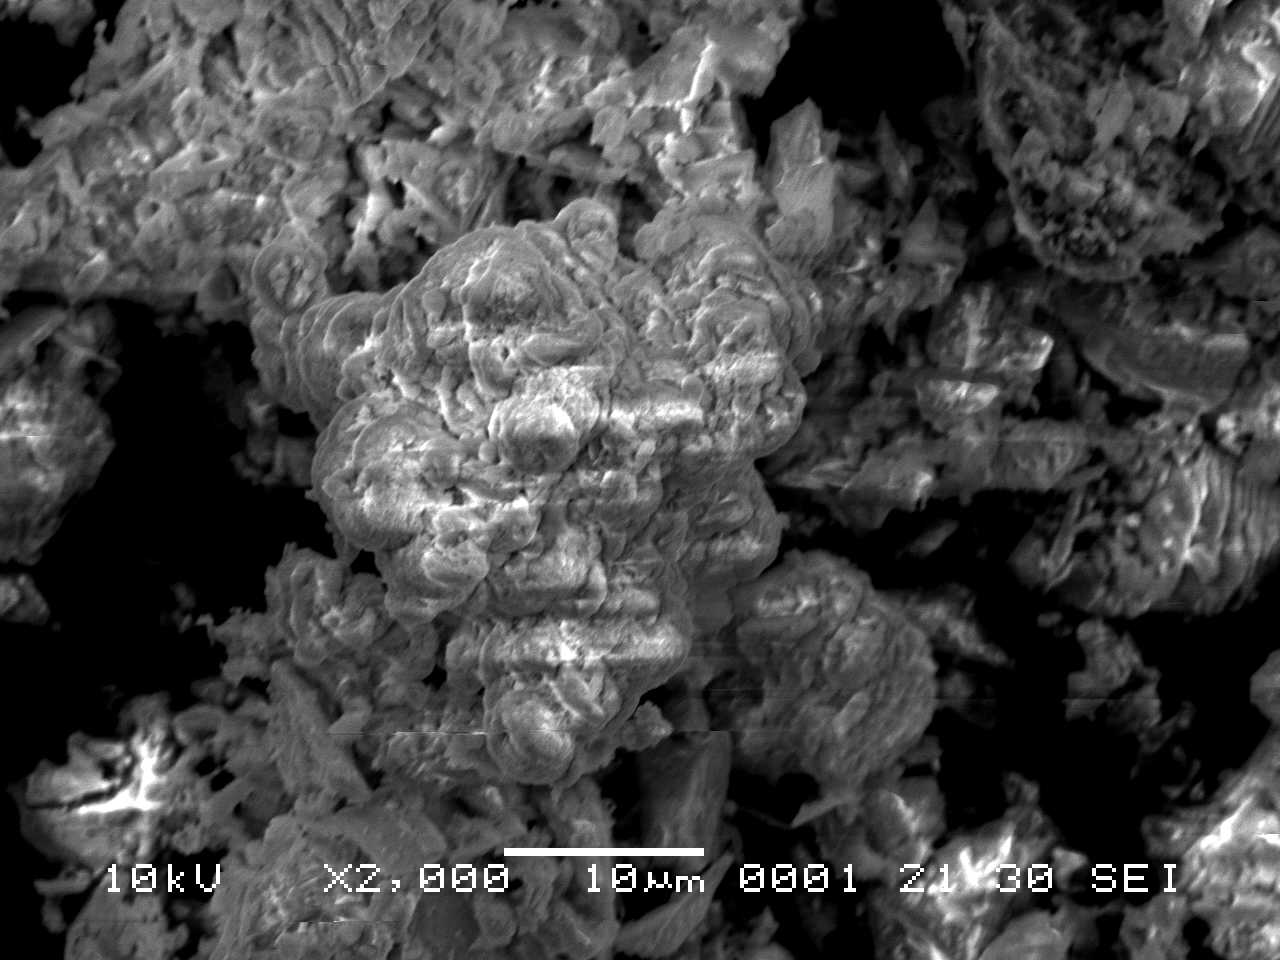
\includegraphics[width=\linewidth]{AzOp_x2000_4_150321}
\end{minipage}
\caption[SEM images: Sample AzOp, azurite]{SEM images: Sample AzOp, azurite. Magnification: 2000x}
\label{fig:azop_sem_3}
\end{figure}

% ************************************************     Fitz1     *******************************************************************
\todo{can you use NLP or ML to do this kind of pattern recognization?? this could be good to look into further.}

\textit{Figures \ref{fig:Fitz1_sem_1}} and \textit{Figure \ref{fig:Fitz1_sem_2}} show sample Fitz1 at magnifications from 250x to 2500x. This sample is described as blue verditer, suggesting that it is synthetic rather than natural.

At 250x magnification (\textit{Figure \ref{fig:Fitz1_sem_1}}, left), small uniform particles are seen. These appear generally circular and far more consistent in size and shape than the samples discussed thus far. At 750x magnification (\textit{Figure \ref{fig:Fitz1_sem_1}}, right), it is possible to qualitatively assess the diameter of particles as consistently < 5 $\mu$m. Particles resemble the spherical cluster observed in the sample AzOp. There is regularity of both size and shape, but it is difficult to determine whether the particles are flat discs or stacked semicircles occupying more volume.

\begin{figure}[H]
\centering
\begin{minipage}{.45\textwidth}
  \centering
  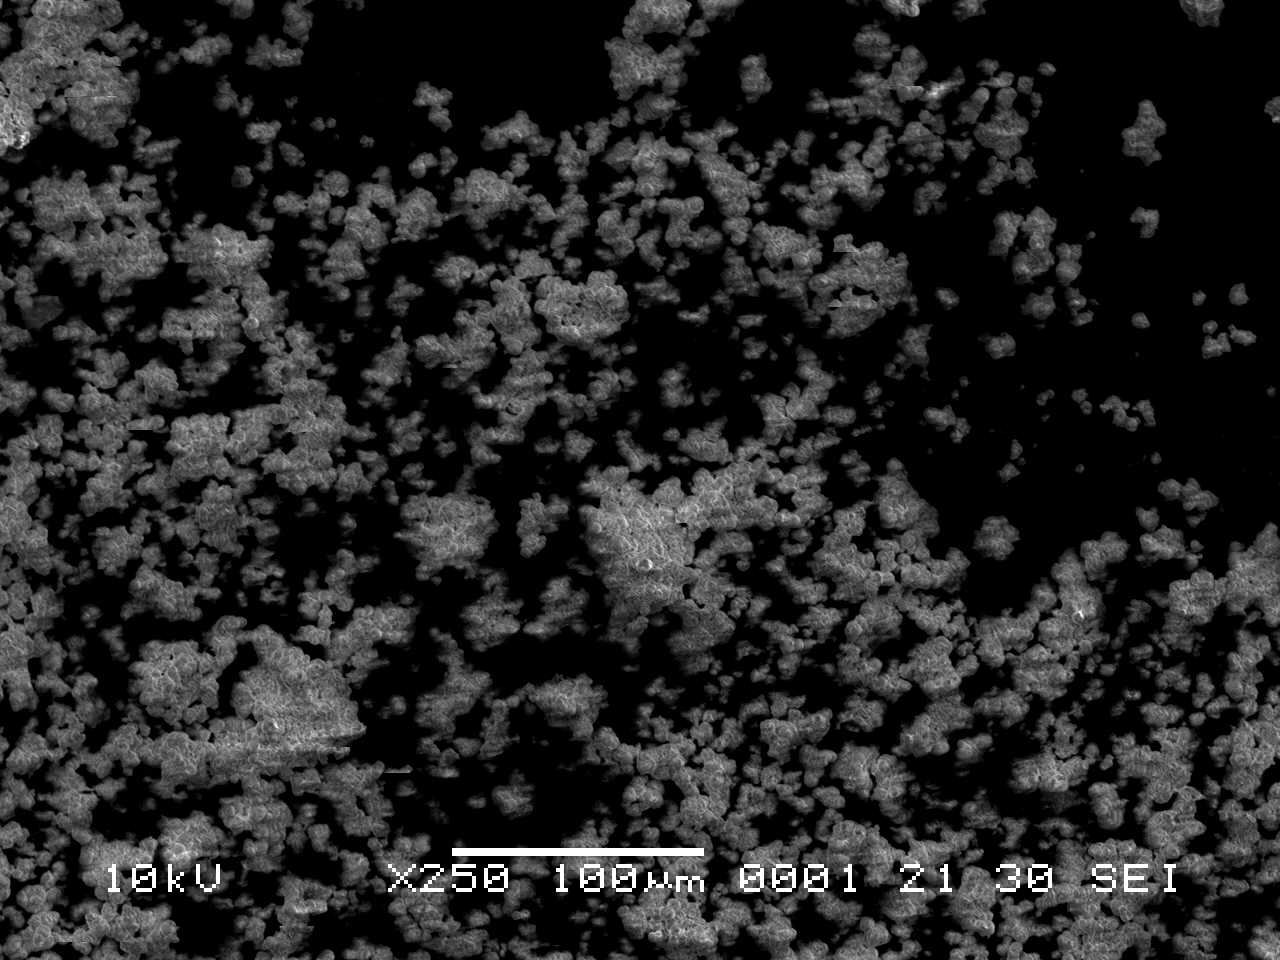
\includegraphics[width=\linewidth]{Fitz1_x250_1_030321}
\end{minipage}
\begin{minipage}{.45\textwidth}
  \centering
  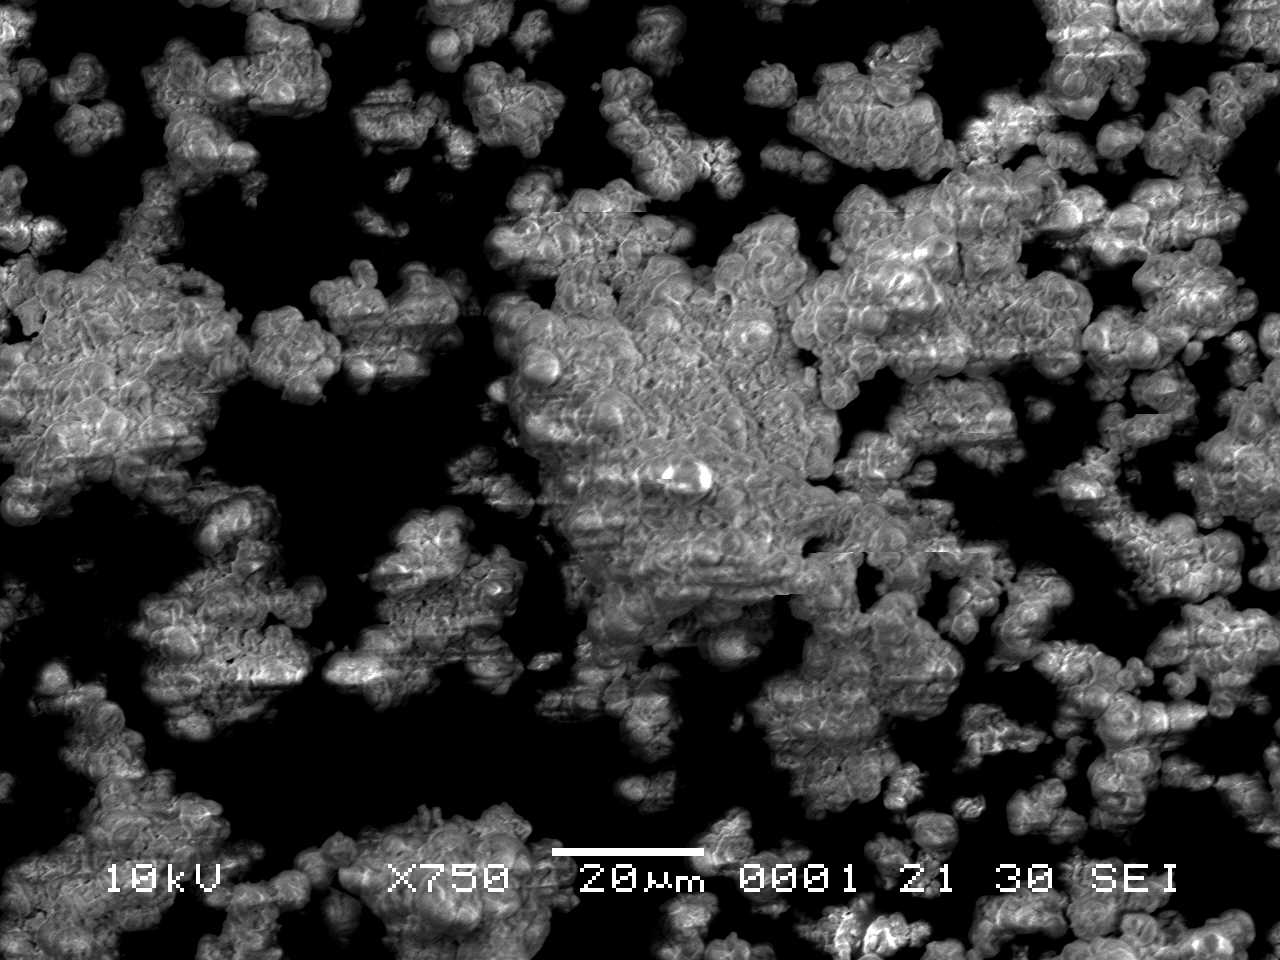
\includegraphics[width=\linewidth]{Fitz1_x750_1_030321}
\end{minipage}
\caption[SEM images: Sample Fitz1, blue verditer]{SEM images: Sample Fitz1, blue verditer. Magnification: \textbf{left)} 250x, \textbf{right)} 750x}
\label{fig:Fitz1_sem_1}
\end{figure}

At 1500x magnification (\textit{Figure \ref{fig:Fitz1_sem_2}}, left), there are clearly spherical particles. These have formed aggregates, though it is not clear whether individual particles could be separated back out of the larger clusters. The size is similar to the spherical cluster in the AzOp sample. The surface also looks slightly pocked or porous. 

The image shown at 2500x magnification (\textit{Figure \ref{fig:Fitz1_sem_2}}, right) is of lower quality than that at 1500x due to surface charging and jumping which made slower acquisitions unsuccessful. The faster acquisition does appear to flatten the image somewhat, which is important to consider since this makes it difficult to judge the volume of particles. There appear to be relatively flat aggregations of approximately circular particles with diameters of approximately 5 $\mu$m.

\begin{figure}[H]
\centering
\begin{minipage}{.45\textwidth}
  \centering
  \includegraphics[width=\linewidth]{Fitz1_x1500_2_030321}
\end{minipage}
\begin{minipage}{.45\textwidth}
  \centering
  \includegraphics[width=\linewidth]{Fitz1_x2500_1_030321}
\end{minipage}
\caption[SEM images: Sample Fitz1, blue verditer]{SEM images: Sample Fitz1, blue verditer. Magnification: \textbf{left)} 1500x, \textbf{right)} 2500x}
\label{fig:Fitz1_sem_2}
\end{figure}

% ************************************************     KE3     *******************************************************************

\textit{Figures \ref{fig:KE3_sem_1}} and \textit{Figure \ref{fig:KE3_sem_2}} show sample KE3 at magnifications from 250x to 2000x. The sample is described as light verditer bice. Verditer suggests a synthetic origin, while bice is used to refer to both natural and synthetic blue pigments. Tentatively, this sample is assumed to be synthetic based on this information.

The image collected at 250x magnification (\textit{Figure \ref{fig:KE3_sem_1}}, left) showed minor issues with charging. Very small particles are present with minimal aggregation. These appear very uniform in size and slightly spherical. At 750x magnification (\textit{Figure \ref{fig:KE3_sem_1}}, right), the uniformity of the particles is more easily observed. They are fairly symmetric, but more angular than sample Fitz1. There are some areas of needle-like structures as well as stacks of spherical or octagonal particles forming small aggregates.

\begin{figure}[H]
\centering
\begin{minipage}{.45\textwidth}
  \centering
  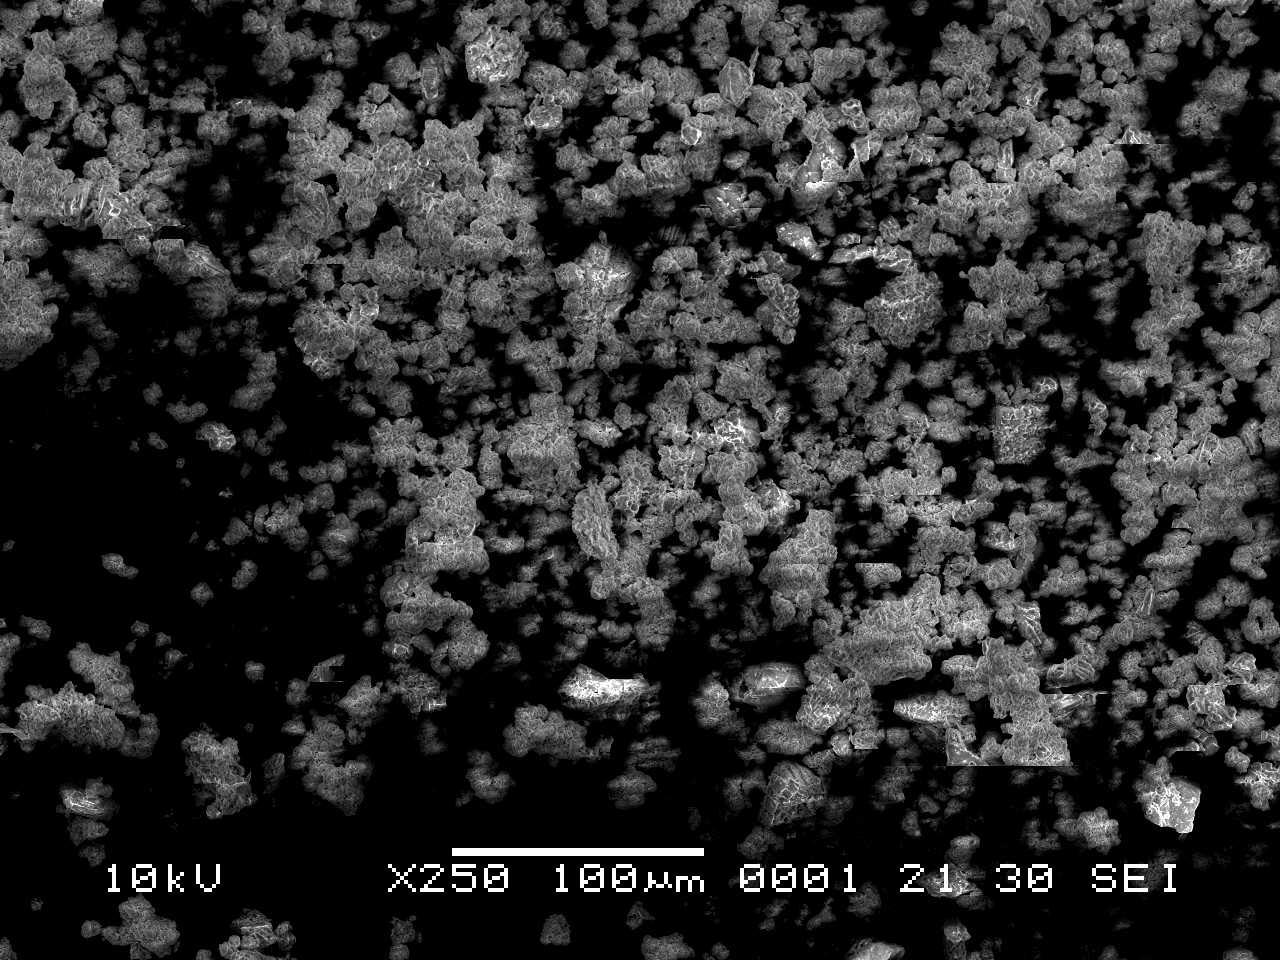
\includegraphics[width=\linewidth]{KE3_x250_1_050321}
\end{minipage}
\begin{minipage}{.45\textwidth}
  \centering
  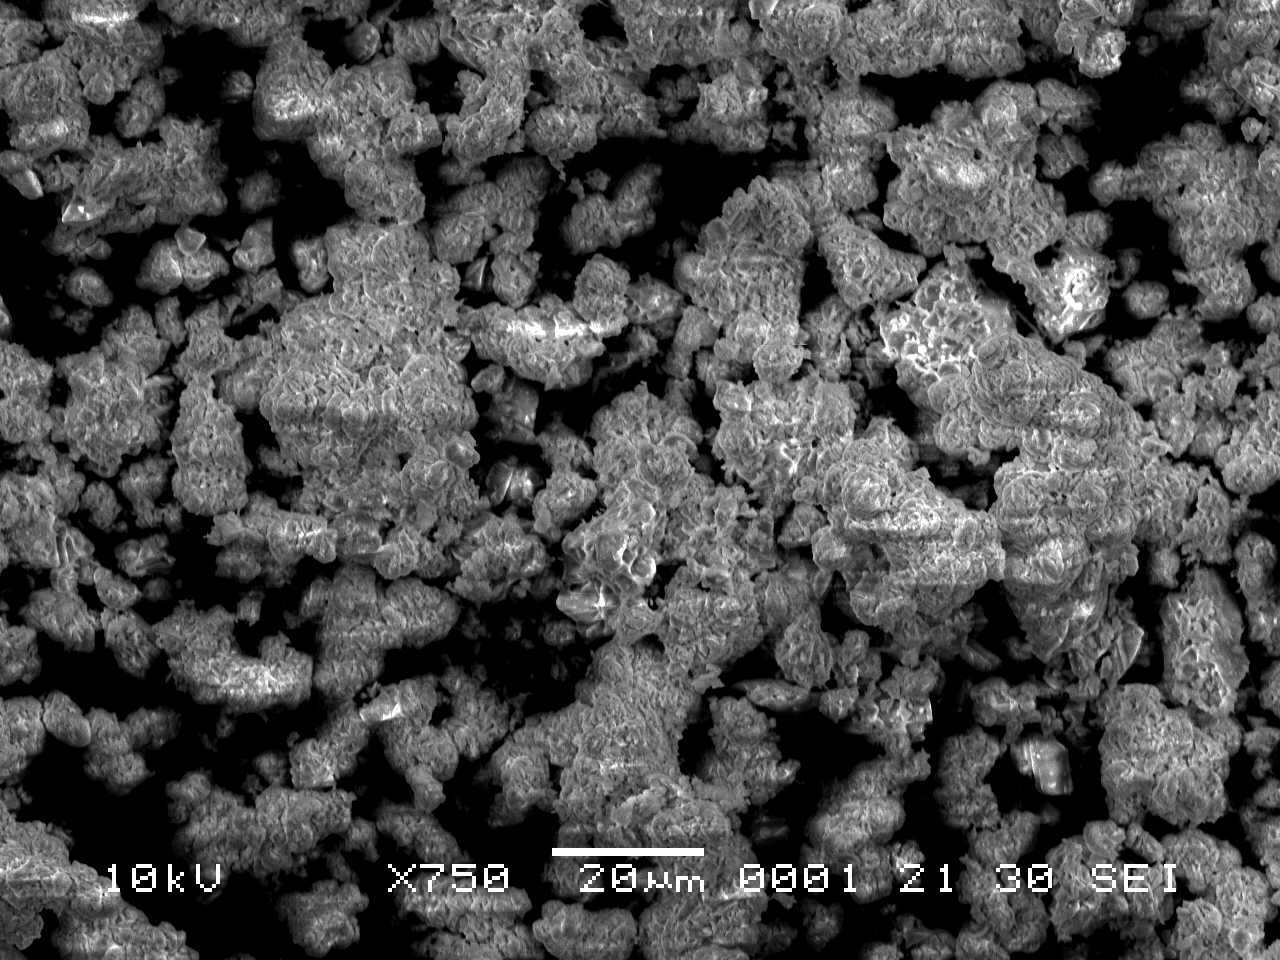
\includegraphics[width=\linewidth]{KE3_x750_3_050321}
\end{minipage}
\caption[SEM images: Sample KE3, light verditer bice]{SEM images: Sample KE3, light verditer bice. Magnification: \textbf{left)} 250x, \textbf{right)} 750x}
\label{fig:KE3_sem_1}
\end{figure}

The approximate particle size can be approximated to 5-10 $\mu$m from the image collected at 1500x magnification (\textit{Figure \ref{fig:KE3_sem_2}}, left). The surfaces appear more porous or pocked than sample Fitz1, but particles are more spherical and uniform than samples from natural origin. At 2000x magnification (\textit{Figure \ref{fig:KE3_sem_2}}, right), spheres are observed. There is significant texture on the surface that is quite fine especially around the edges of particles, and this texture appears rougher than that of sample Fitz1. This may be due, though, to poorer image quality of the Fitz1 sample.

\begin{figure}[H]
\centering
\begin{minipage}{.45\textwidth}
  \centering
  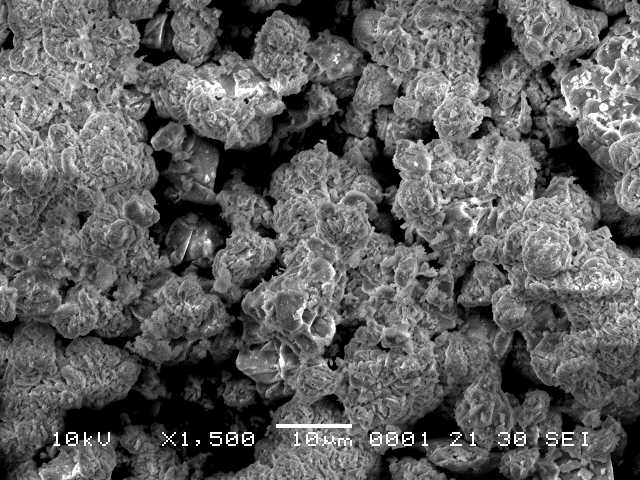
\includegraphics[width=\linewidth]{KE3_x1500_1_050321}
\end{minipage}
\begin{minipage}{.45\textwidth}
  \centering
  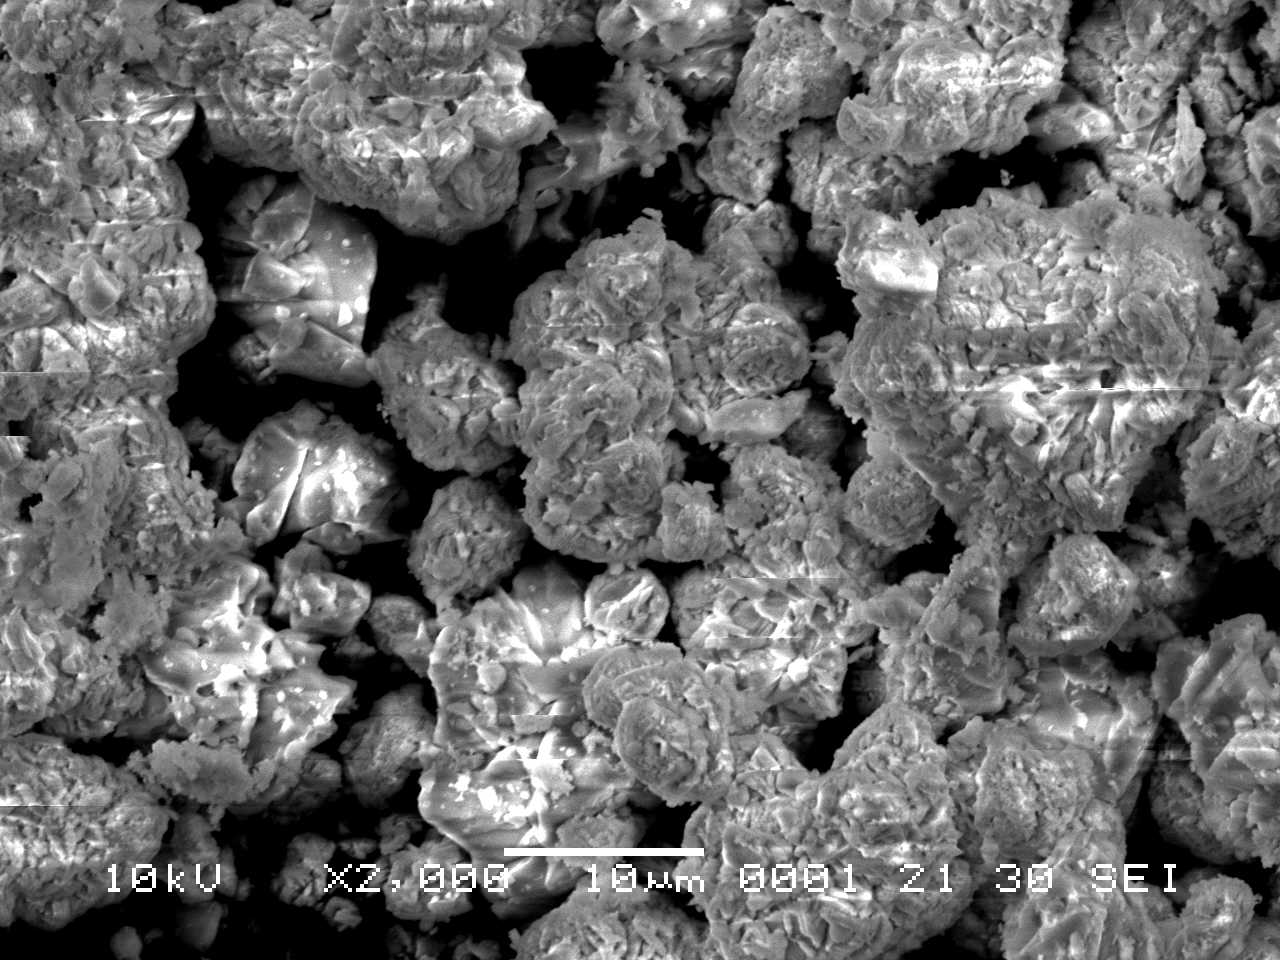
\includegraphics[width=\linewidth]{KE3_x2000_2_050321}
\end{minipage}
\caption[SEM images: Sample KE3, light verditer bice]{SEM images: Sample KE3, light verditer bice. Magnification: \textbf{left)} 1500x, \textbf{right)} 2000x}
\label{fig:KE3_sem_2}
\end{figure}

% ************************************************     KE4     *******************************************************************

\textit{Figures \ref{fig:KE4_sem_1}} and \textit{Figure \ref{fig:KE4_sem_2}} show sample KE4 at magnifications from 250x to 2000x. KE4 is labelled as blue bice, which is an ambiguous description, so it is inconclusive whether this sample was prepared naturally or synthetically.

\textit{Figure \ref{fig:KE4_sem_1}} (left) shows KE4 at 250x magnification. Larger particles on the order of 50 $\mu$m are visible, as are significantly smaller particles on the order of 5 $\mu$m. At 750x magnification (\textit{Figure \ref{fig:KE4_sem_1}}, right), fine needle-like structure is visible similar to that of sample HKI natural azurite. At the same time, there are also rounder structures that resemble Fitz1. 

\begin{figure}[H]
\centering
\begin{minipage}{.45\textwidth}
  \centering
  \includegraphics[width=\linewidth]{KE4_x250_1_030321}
\end{minipage}
\begin{minipage}{.45\textwidth}
  \centering
  \includegraphics[width=\linewidth]{KE4_x750_1_030321}
\end{minipage}
\caption[SEM images: Sample KE4, blue bice]{SEM images: Sample KE4, blue bice. Magnification: \textbf{left)} 250x, \textbf{right)} 750x}
\label{fig:KE4_sem_1}
\end{figure}

\textit{Figure \ref{fig:KE4_sem_2}} (left) shows KE4 at 1000x magnification, where the fine structure resembling needles or feathers is very clear. These structures are not oriented in any way, and appear randomly assembled. \textit{Figure \ref{fig:KE4_sem_2}} (right) shows KE4 at 2000x magnification. The image is focused on the flat side of a larger particle (or aggregate) with many smaller particles attached to or resting on the surface. There are also pockmarks or cavities observed. This sample is ambiguous as it shows characteristics of known natural as well as synthetic samples.

\begin{figure}[H]
\centering
\begin{minipage}{.45\textwidth}
  \centering
  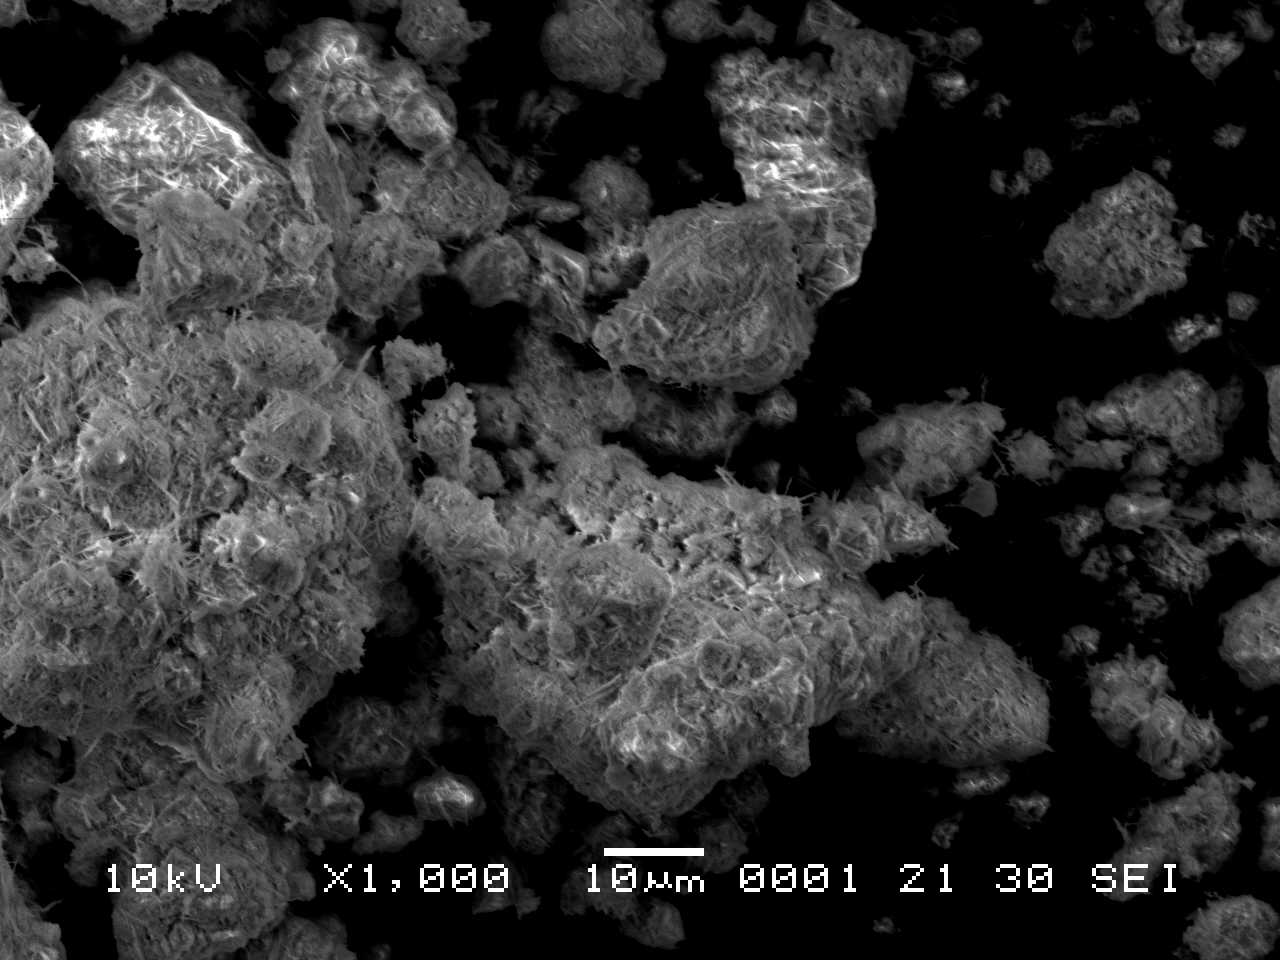
\includegraphics[width=\linewidth]{KE4_x1000_1_030321}
\end{minipage}
\begin{minipage}{.45\textwidth}
  \centering
  \includegraphics[width=\linewidth]{KE4_x2000_1_030321}
\end{minipage}
\caption[SEM images: Sample KE4, blue bice]{SEM images: Sample KE4, blue bice. Magnification: \textbf{left)} 1000x, \textbf{right)} 2000x}
\label{fig:KE4_sem_2}
\end{figure}

% ************************************************     KE5     *******************************************************************

\textit{Figures \ref{fig:KE5_sem_1}} and \textit{Figure \ref{fig:KE5_sem_2}} show sample KE5 at magnifications from 250x to 2000x. KE5 is described as blue verditer, strongly suggesting a synthetic origin.

\textit{Figure \ref{fig:KE5_sem_1}} (left) shows KE5 at 250x magnification. Small circular particles of uniform size and shape are observed. \textit{Figure \ref{fig:KE5_sem_1}} (right) shows KE5 at 750x magnification. At this magnification, larger aggregates of approximately 80 $\mu$m are clearly seen to be formed from smaller particles. This is very similar to the appearance of Fitz1 at the same magnification. The appearance also brings to mind the crystal formation of desert rose gypsum, characterized by intersecting flat discs forming circular or semicircular three dimensional structures.%~\autocite{hope_gypsum} 

\textit{Figure \ref{fig:KE5_sem_2}} shows KE5 at 1500x magnification (left) and 2000x magnification (right). The circular character of particles is very clearly observed in these images.

\begin{figure}[H]
\centering
\begin{minipage}{.45\textwidth}
  \centering
  \includegraphics[width=\linewidth]{KE5_x250_2_050321}
\end{minipage}
\begin{minipage}{.45\textwidth}
  \centering
  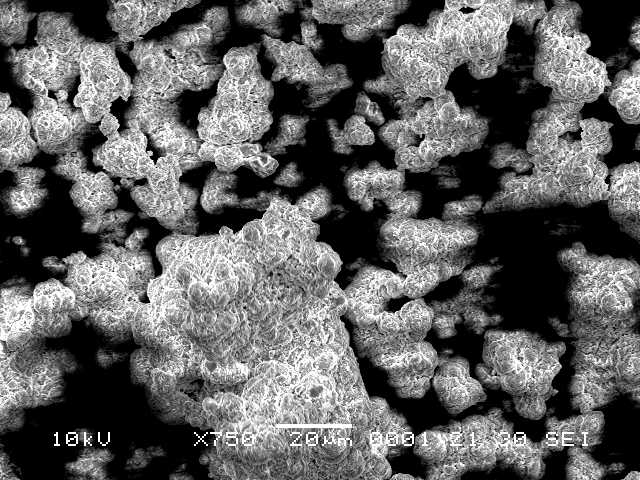
\includegraphics[width=\linewidth]{KE5_x750_1_050321}
\end{minipage}
\caption[SEM images: Sample KE5, blue verditer]{SEM images: Sample KE5, blue verditer. Magnification: \textbf{left)} 250x, \textbf{right)} 750x}
\label{fig:KE5_sem_1}
\end{figure}

\begin{figure}[H]
\centering
\begin{minipage}{.45\textwidth}
  \centering
  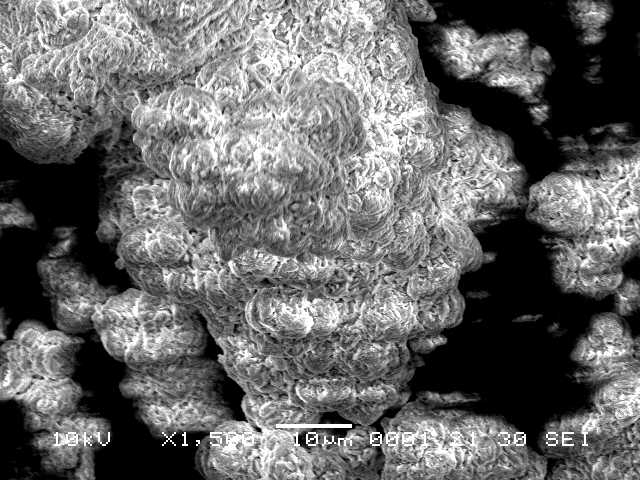
\includegraphics[width=\linewidth]{KE5_x1500_1_050321}
\end{minipage}
\begin{minipage}{.45\textwidth}
  \centering
  \includegraphics[width=\linewidth]{KE5_x2000_2_050321}
\end{minipage}
\caption[SEM images: Sample KE5, blue verditer]{SEM images: Sample KE5, blue verditer. Magnification: \textbf{left)} 1500x, \textbf{right)} 2000x}
\label{fig:KE5_sem_2}
\end{figure}

\subsubsection[Particle size distribution of natural and artificial azurite]{Particle size distribution of natural and artificial azurite}
\label{subsubsection3.1.1.1}

SEM images at 750x magnification were collected from edges of loose pigments samples used for SEM analysis above where particles were most loosely dispersed. The two samples selected, HKI natural azurite and Fitz 1, were selected on the basis of their known sources as well as significantly different morphology. These images were processed in Fiji ImageJ (XXXX version) by increasing contrast and manually thresholding (shown in \textit{Figures \ref{} and \ref{}}) followed by manual selection of maximum lengths and measurement using the image scale bar. 

Five images of Fitz 1 were analyzed, with n(particles) = 102. Five images of HKI natural azurite were analyzed, with n(particles) = 127. There is undoubtedly some bias in selected particles due to the difficulty of defining edges in the images, and this may affect the spread of results. Examples of the original SEM image (left) and the thresholded binary image (right, used for measurements) are shown for Fitz 1 in \textit{Figure \ref{fig:imageJ_fitz1}} and for HKI natural azurite in \textit{Figure \ref{fig:imageJ_hki}}. 

\begin{figure}[H]
\centering
\begin{minipage}{.45\textwidth}
  \centering
  \includegraphics[width=\linewidth]{Fitz1_x750_5_130521}
\end{minipage}
\begin{minipage}{.45\textwidth}
  \centering
  \includegraphics[width=\linewidth]{Fitz1_x750_5_130521_BW}
\end{minipage}
\caption[Particle size analysis: Sample Fitz 1]{Particle size analysis: Sample Fitz 1. \textbf{Left)} original SEM image, \textbf{Right)} thresholded binary image.}
\label{fig:imageJ_fitz1}
\end{figure}

\begin{figure}[H]
\centering
\begin{minipage}{.45\textwidth}
  \centering
  \includegraphics[width=\linewidth]{HKI_natural_azurite_x750_1_130521}
\end{minipage}
\begin{minipage}{.45\textwidth}
  \centering
  \includegraphics[width=\linewidth]{HKI_natural_azurite_x750_1_130521-2_BW}
\end{minipage}
\caption[Particle size analysis: Sample HKI natural azurite]{Particle size analysis: Sample HKI natural azurite. \textbf{Left)} original SEM image, \textbf{Right)} thresholded binary image.}
\label{fig:imageJ_hki}
\end{figure}

The measurements from each sample image were combined and analysed using R (version XXXX) to produce a histogram of the frequency of length measurements (bin size = 1 $\mu$m) for each sample, shown in \textit{Figure \ref{fig:histogram_length}}. Based on the different particle morphologies, it would be reasonable to expect that the particle size distribution would differ between samples. Additionally, the presence of a bimodal distribution in the histogram might indicate the formation of aggregates of a specific size from single particles. 

The length distributions of Fitz 1 and HKI natural azurite do not show significant differences. Both show a high frequency of particles with lengths around 5 $\mu$m, with a low frequency of particles or clusters above 10 $\mu$m. Sample Fitz 1 does appear to have several particles of length around 15 $\mu$m, which is absent in HKI natural azurite. This could suggest that aggregates are forming at more consistent sizes than in sample HKI natural azurite. Overall, though, these two samples are statistically very similar in this analysis. \textit{Table \ref{table:r_stats}} contains descriptive statistics, and it is notable how similar the means and medians are between samples.  

\begin{figure}[H]
\centering
\begin{minipage}{.45\textwidth}
  \centering
  \includegraphics[width=\linewidth]{hist_fitz1}
\end{minipage}
\begin{minipage}{.45\textwidth}
  \centering
  \includegraphics[width=\linewidth]{hist_hki}
\end{minipage}
\caption[Particle size analysis: Sample HKI natural azurite]{Particle size analysis: Sample HKI natural azurite. \textbf{Left)} Fitz 1, \textbf{Right)} HKI natural azurite.}
\label{fig:histogram_length}
\end{figure}

\begin{table}[H]
\caption{Descriptive statistics: Fitz 1, HKI natural azurite}
\centering
\label{table:r_stats}
\begin{tabular}{c c c c}
\toprule
Reference sample & Mean & Median & Range \\
\midrule
HKI natural azurite & 5.437 & 8.583 & 1.177 - 52.176 \\
Fitz 1 & 5.878 & 8.683 & 2.414 - 38.367 \\
\bottomrule
\end{tabular}
\end{table}

%fitz 1
%Median : 5.878  
%Mean   : 8.683
%range 2.414 to 38.367
% hki 
%Median : 5.437  
%Mean   : 8.583
%range 1.177 to 52.176

% *******************************************************************************************************************************
% *******************************************************************************************************************************
% *******************************************************************************************************************************

\subsection[Malachite and green verditer]{Malachite and green verditer}
\label{subsection3.1.2}

% ************************************************     Ma1     *******************************************************************

\textit{Figures \ref{fig:Ma1_sem_1}-\ref{fig:Ma1_sem_4}} show sample Ma1 at magnifications from 250x to 4000x. This sample is natural malachite.

At low magnification (200-250x) as shown in \textit{Figure \ref{fig:Ma1_sem_1}}, the sample appears extremely powdery and fine. The size and shape of particles are extremely irregular in both size and shape. 

\begin{figure}[H]
\centering
\begin{minipage}{.45\textwidth}
  \centering
  \includegraphics[width=\linewidth]{Ma1_x200_1_240221}
\end{minipage}
\begin{minipage}{.45\textwidth}
  \centering
  \includegraphics[width=\linewidth]{Ma1_x250_2_160321}
\end{minipage}
\caption[SEM images: Sample Ma1, malachite]{SEM images: Sample Ma1, malachite. Magnification: \textbf{left)} 200x, \textbf{right)} 250x}
\label{fig:Ma1_sem_1}
\end{figure}

At 750x magnification (\textit{Figure \ref{fig:Ma1_sem_2}}, left), the extreme irregularity of particles is apparent. Particles have extremely rough and choppy edges, and these irregular shapes closely resemble those of natural azurite samples in terms of their roughness and sharpness. There are few aggregates or clumps that are larger than 20 $\mu$m. At 1500x magnification (\textit{Figure \ref{fig:Ma1_sem_2}}, right), the texture of surfaces of the large (approx. 20 $\mu$m) aggregates is observed. It consists of particles of less than 5 $\mu$m across. 
\begin{figure}[H]
\centering
\begin{minipage}{.45\textwidth}
  \centering
  \includegraphics[width=\linewidth]{Ma1_x750_2_160321}
\end{minipage}
\begin{minipage}{.45\textwidth}
  \centering
  \includegraphics[width=\linewidth]{Ma1_x1500_2_160321}
\end{minipage}
\caption[SEM images: Sample Ma1, malachite]{SEM images: Sample Ma1, malachite. Magnification: \textbf{left)} 750x, \textbf{right)} 1500x}
\label{fig:Ma1_sem_2}
\end{figure}

\textit{Figure \ref{fig:Ma1_sem_3}} shows two areas of the sample at 2500x magnification. The sample is disordered and heterogeneous. While it is possible that this is due to grinding the pigment during preparation, \textit{Figure \ref{fig:Ma1_sem_4}} shows further disorder at 3000x and 4000x magnification. Here, many particles under 1 $\mu$m across are present, with extremely uneven borders. These are unambiguously single particles rather than surface roughness on a larger plane.


\begin{figure}[H]
\centering
\begin{minipage}{.45\textwidth}
  \centering
  \includegraphics[width=\linewidth]{Ma1_x2500_2_160321}
\end{minipage}
\begin{minipage}{.45\textwidth}
  \centering
  \includegraphics[width=\linewidth]{Ma1_x2500_3_160321}
\end{minipage}
\caption[SEM images: Sample Ma1, malachite]{SEM images: Sample Ma1, malachite. Magnification: 2500x}
\label{fig:Ma1_sem_3}
\end{figure}

\begin{figure}[H]
\centering
\begin{minipage}{.45\textwidth}
  \centering
  \includegraphics[width=\linewidth]{Ma1_x3000_2_160321}
\end{minipage}
\begin{minipage}{.45\textwidth}
  \centering
  \includegraphics[width=\linewidth]{Ma1_x4000_1_160321}
\end{minipage}
\caption[SEM images: Sample Ma1, malachite]{SEM images: Sample Ma1, malachite. Magnification: \textbf{left)} 3000x, \textbf{right)} 4000x}
\label{fig:Ma1_sem_4}
\end{figure}

% ************************************************     KE1a     *******************************************************************

\textit{Figures \ref{fig:KE1a_sem_1}} shows sample KE1a at magnifications 250x (left) and 750x (right). The name of Ke1a, green bice, is ambiguous and could refer to a natural or an artificial sample.

At 250x magnification, small particles form aggregations of approximately 25-50 $\mu$m. The image at 750x magnification is poor quality, and charging prevented use of higher magnifications. The shapes of particles do appear to be squared-off circles with some degree of uniformity. \mynote{(there may be a better way to say this)} They are not, however, spherical like several of the blue pigment samples discussed above. 

This sample is qualitatively more uniform than sample Ma1, and more spherical, but it is more challenging to draw clear conclusions about morphological differences between natural and synthetic green samples compared to blue. There is a much smaller sample size in the reference samples available, as well as ambiguity in sample source, but this also may just mean that green samples do not show marked morphology changes depending on production process.

\begin{figure}[H]
\centering
\begin{minipage}{.45\textwidth}
  \centering
  \includegraphics[width=\linewidth]{KE1a_x250_1_040321}
\end{minipage}
\begin{minipage}{.45\textwidth}
  \centering
  \includegraphics[width=\linewidth]{KE1a_x750_2_040321}
\end{minipage}
\caption[SEM images: Sample KE1a, green bice]{SEM images: Sample KE1a, green bice. Magnification: \textbf{left)} 250x, \textbf{right)} 750x}
\label{fig:KE1a_sem_1}
\end{figure}

% ************************************************     KE1b     *******************************************************************

%didnt do this one

% ************************************************     KE2     *******************************************************************

\textit{Figures \ref{fig:KE2_sem_1}} and \textit{\ref{fig:KE2_sem_2}} show sample KE2, green verditer. The sample name strongly suggests a synthetic source. 

In \textit{Figure \ref{fig:KE2_sem_1}}, the sample is shown at 250x (left) and 750x (right) magnifications. At 250x magnification, the sample appears fairly uniform in size and shape. It is very finely ground or naturally consists of small crystals and aggregates. At 750x magnification, particles are very irregularly shaped, sharp, and generally not elongated.

\begin{figure}[H]
\centering
\begin{minipage}{.45\textwidth}
  \centering
  \includegraphics[width=\linewidth]{KE2_250_1_040321}
\end{minipage}
\begin{minipage}{.45\textwidth}
  \centering
  \includegraphics[width=\linewidth]{KE2_x750_1_040321}
\end{minipage}
\caption[SEM images: Sample KE2, green verditer]{SEM images: Sample KE2, green verditer. Magnification: \textbf{left)} 250x, \textbf{right)} 750x}
\label{fig:KE2_sem_1}
\end{figure}

In \textit{Figure \ref{fig:KE2_sem_2}}, the sample is shown at 1500x (left) and 2000x (right) magnifications. It is possible to estimate the particle size at approximately 7-10 $\mu$m in the image at 1500x magnification. At 2000x magnification, there is a lack of texture on the surface of individual particles. The edges of particles are extremely feathery, which is observed in other samples discussed in this section as well.

\begin{figure}[H]
\centering
\begin{minipage}{.45\textwidth}
  \centering
  \includegraphics[width=\linewidth]{KE2_x1500_040321}
\end{minipage}
\begin{minipage}{.45\textwidth}
  \centering
  \includegraphics[width=\linewidth]{Ke2_x2000_1_040321}
\end{minipage}
\caption[SEM images: Sample KE2, green verditer]{SEM images: Sample KE2, green verditer. Magnification: \textbf{left)} 1500x, \textbf{right)} 2000x}
\label{fig:KE2_sem_2}
\end{figure}


% *******************************************************************************************************************************
% *******************************************************************************************************************************
% *******************************************************************************************************************************

\section[Raman Data]{Raman Data}
\label{section3.2}



\section[AFM Data]{AFM Data}
\label{section3.3}
